\newpage
\section{Обработка результатов измерений}
Изобразим спектры при трех разных температурах: $40^\circ C,~ 55^\circ C,~ 70^\circ C$
\begin{figure}[H]%{r}{0.3\linewidth}
\centering
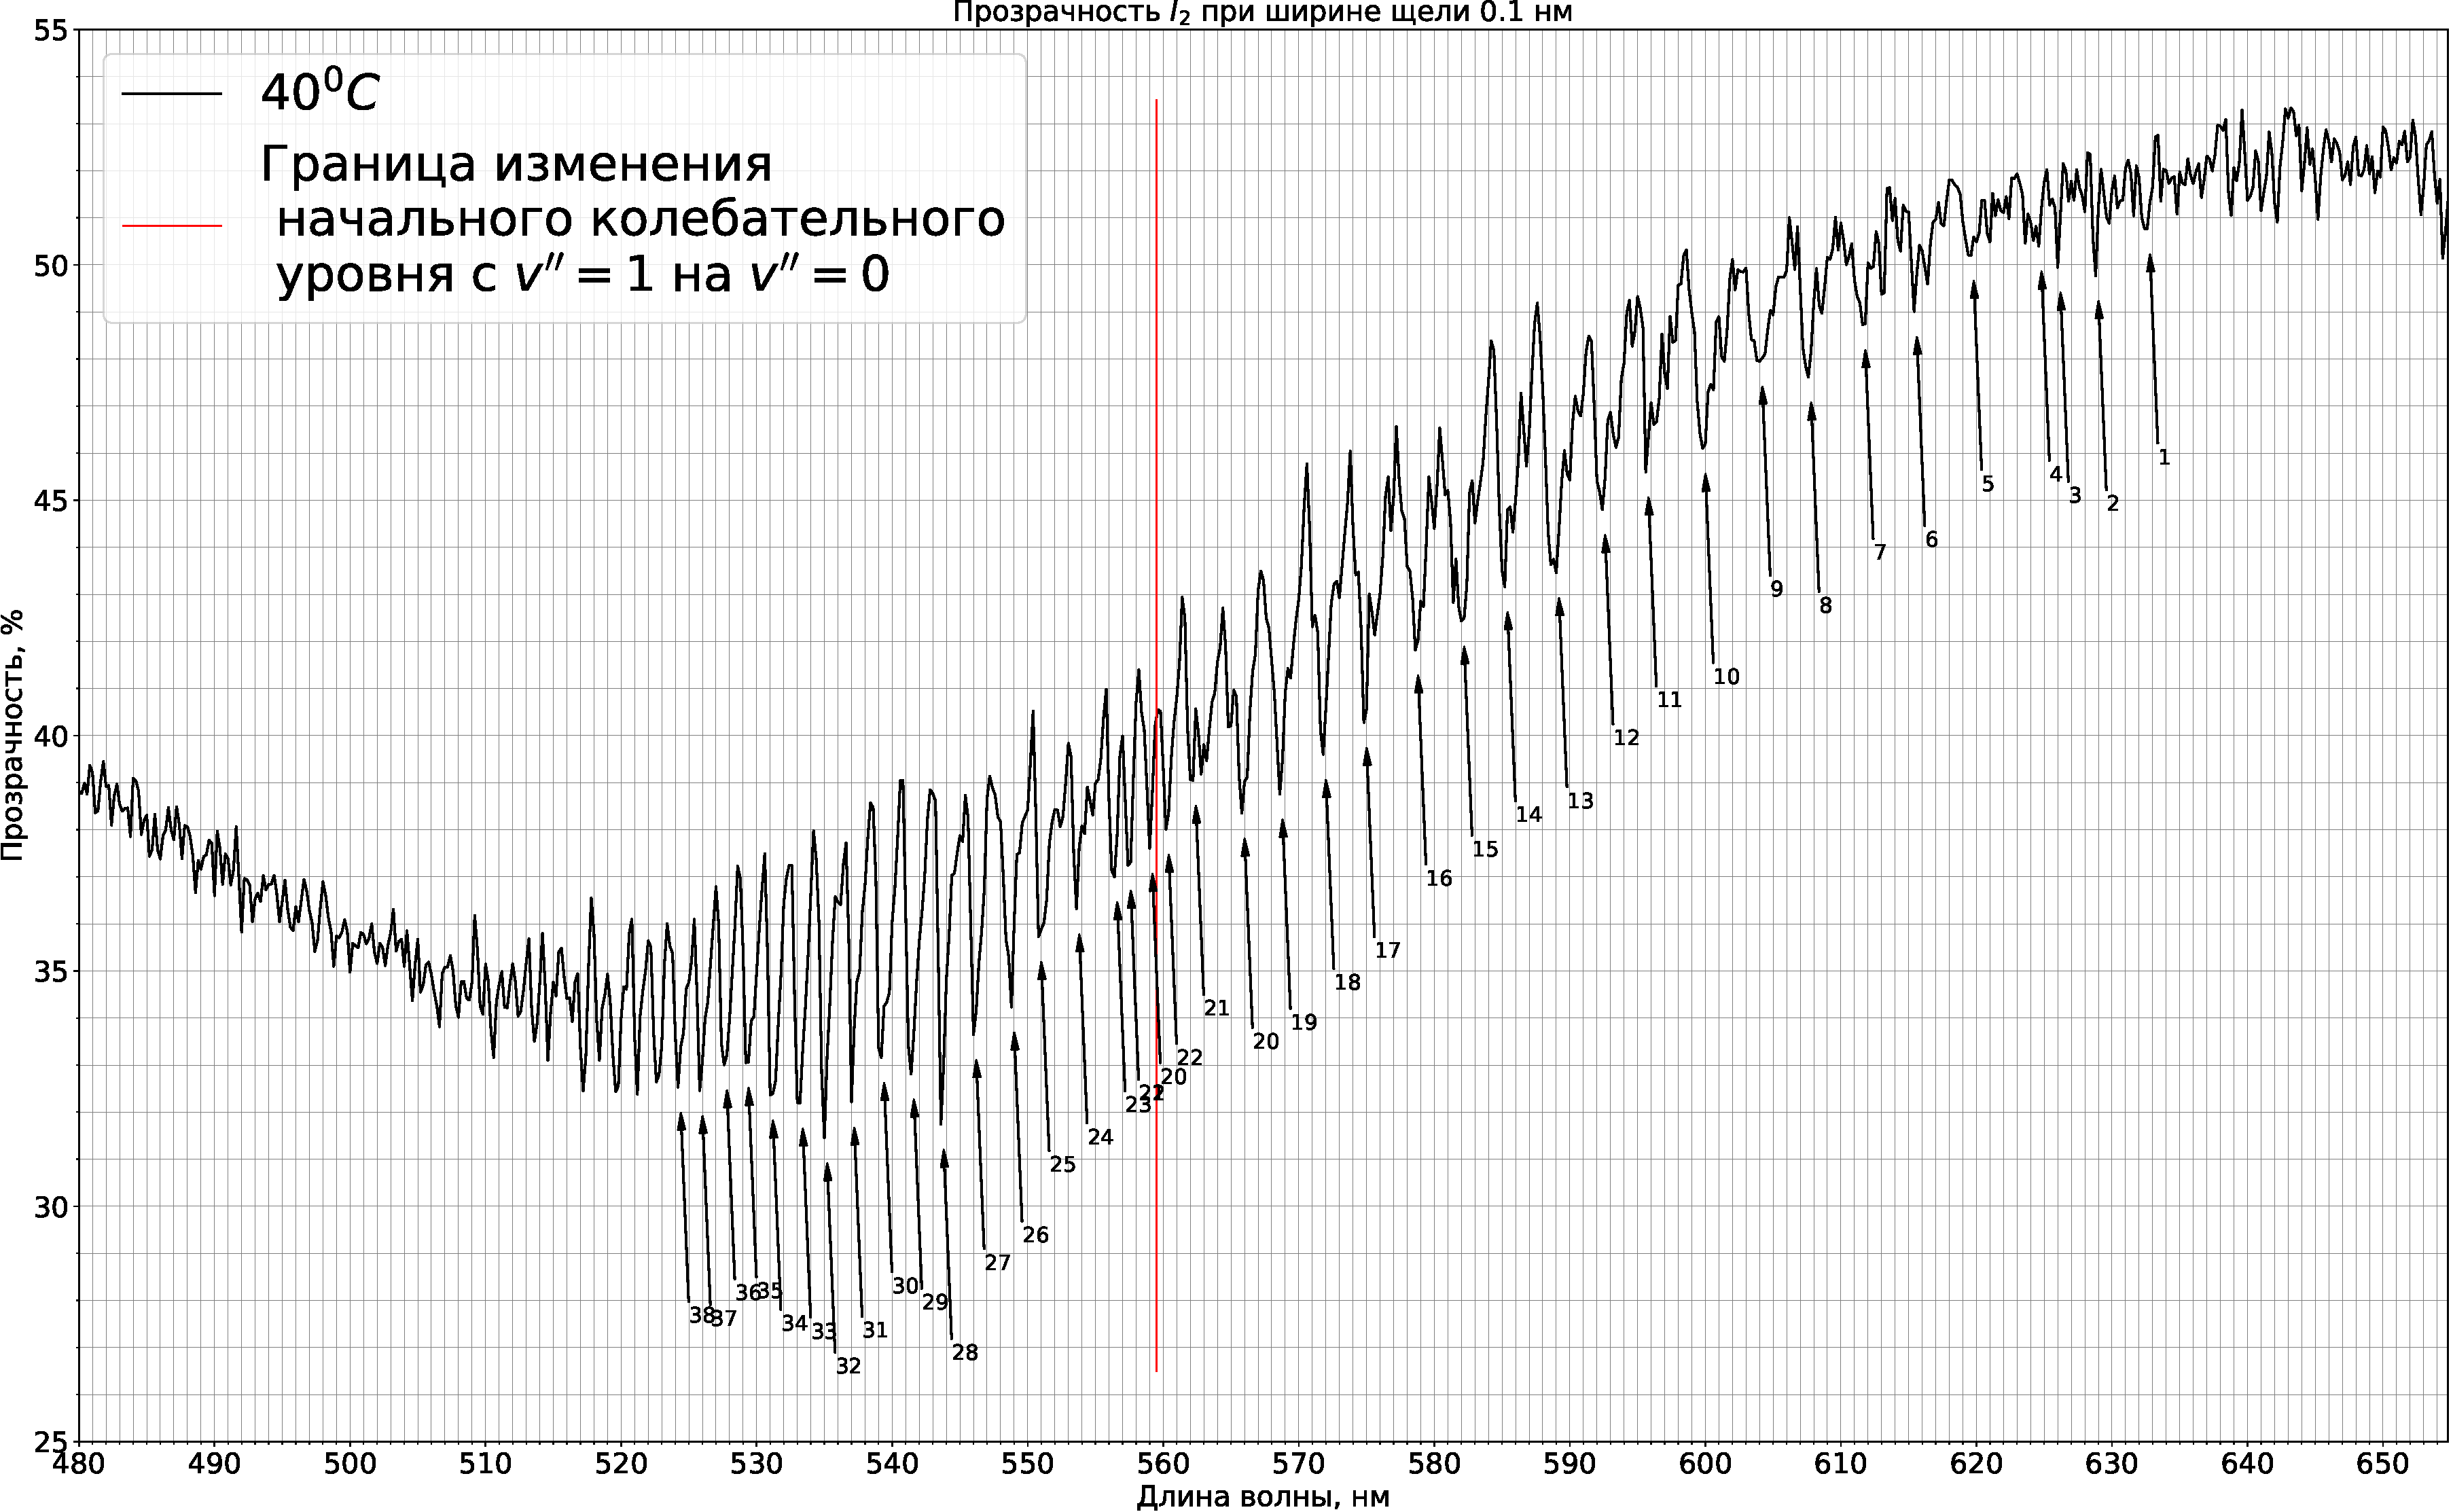
\includegraphics[angle = 90, height=0.87\textheight]{data/40_grad}
\caption{Спектр поглощения молекулы I$_2$, 40 $^\circ C$}
\label{40_graph}
\end{figure}
\begin{figure}[H]%{r}{0.3\linewidth}
\centering
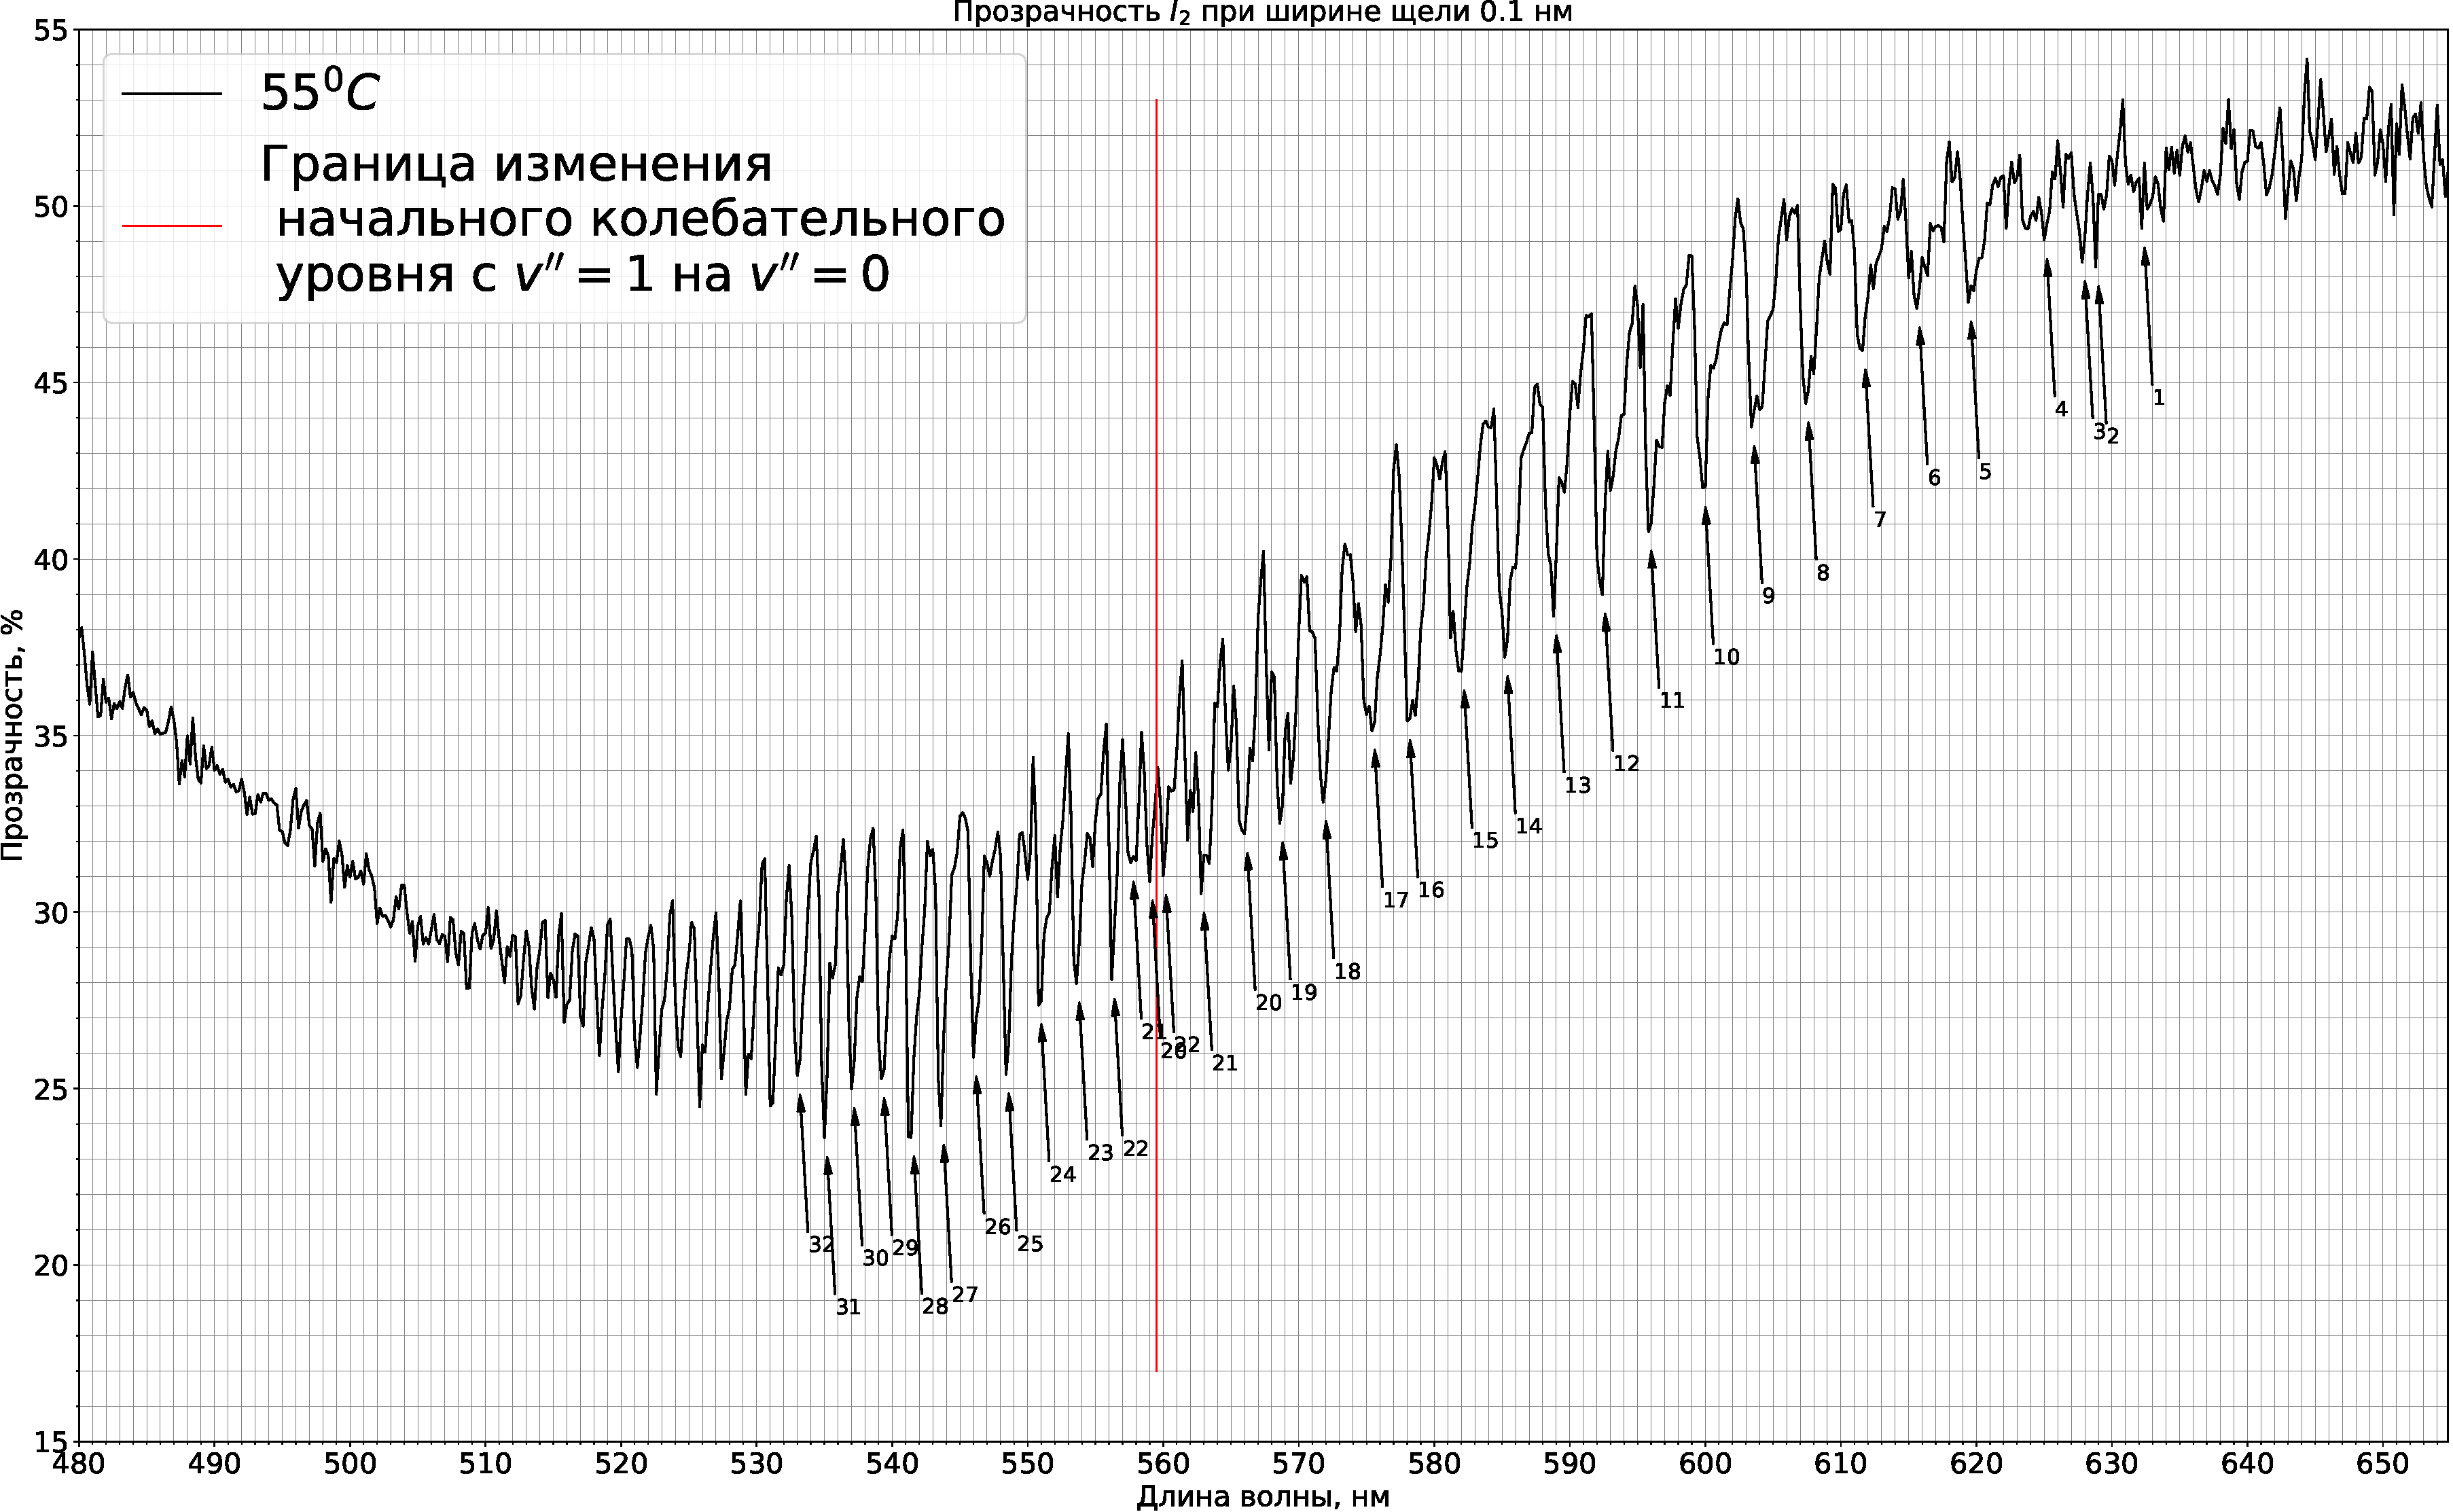
\includegraphics[angle = 90, height=0.95\textheight]{data/55_grad}
\caption{Спектр поглощения молекулы I$_2$, 55 $^\circ C$}
\label{55_graph}
\end{figure}
\begin{figure}[H]%{r}{0.3\linewidth}
\centering
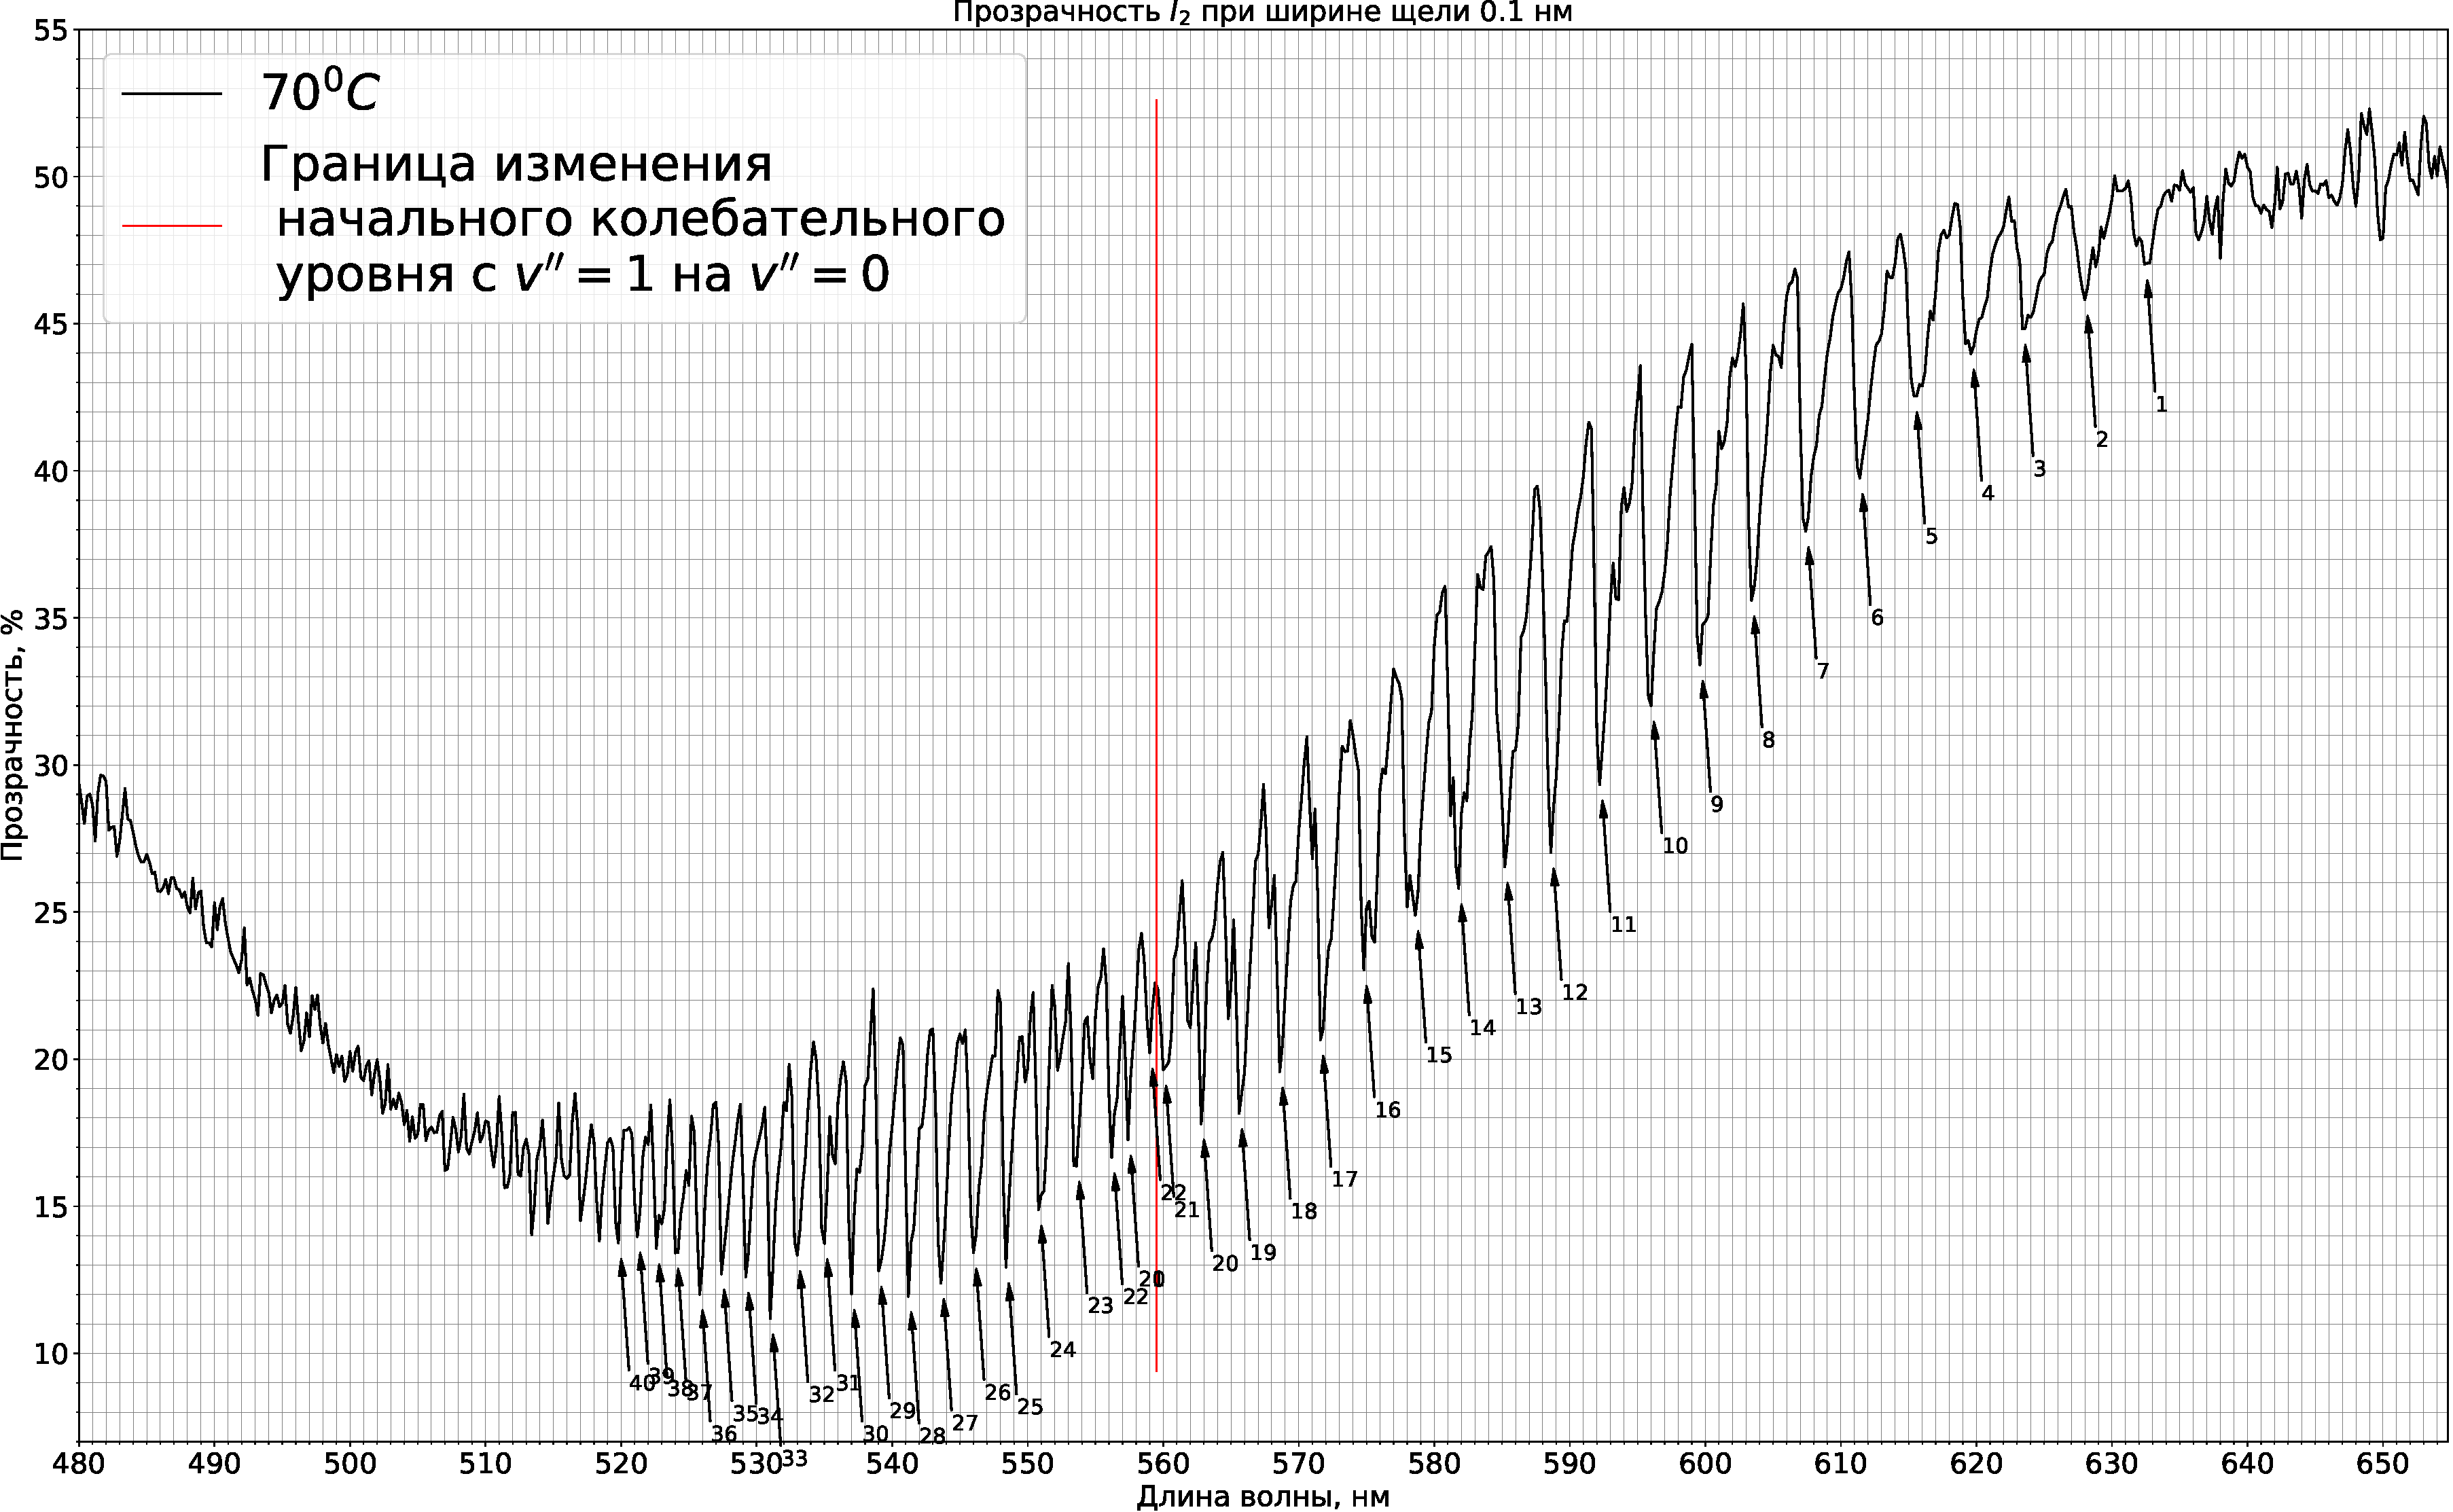
\includegraphics[angle = 90, height=0.95\textheight]{data/70_grad}
\caption{Спектр поглощения молекулы I$_2$, 70 $^\circ C$}
\label{70_graph}
\end{figure}

\newpage
\subsection{Построение таблицы Деландра и анализ спектра}
Изобразим спектры при трех разных температурах на рис. \ref{main_spectrum}.
\begin{figure}[h!]
	\centering
	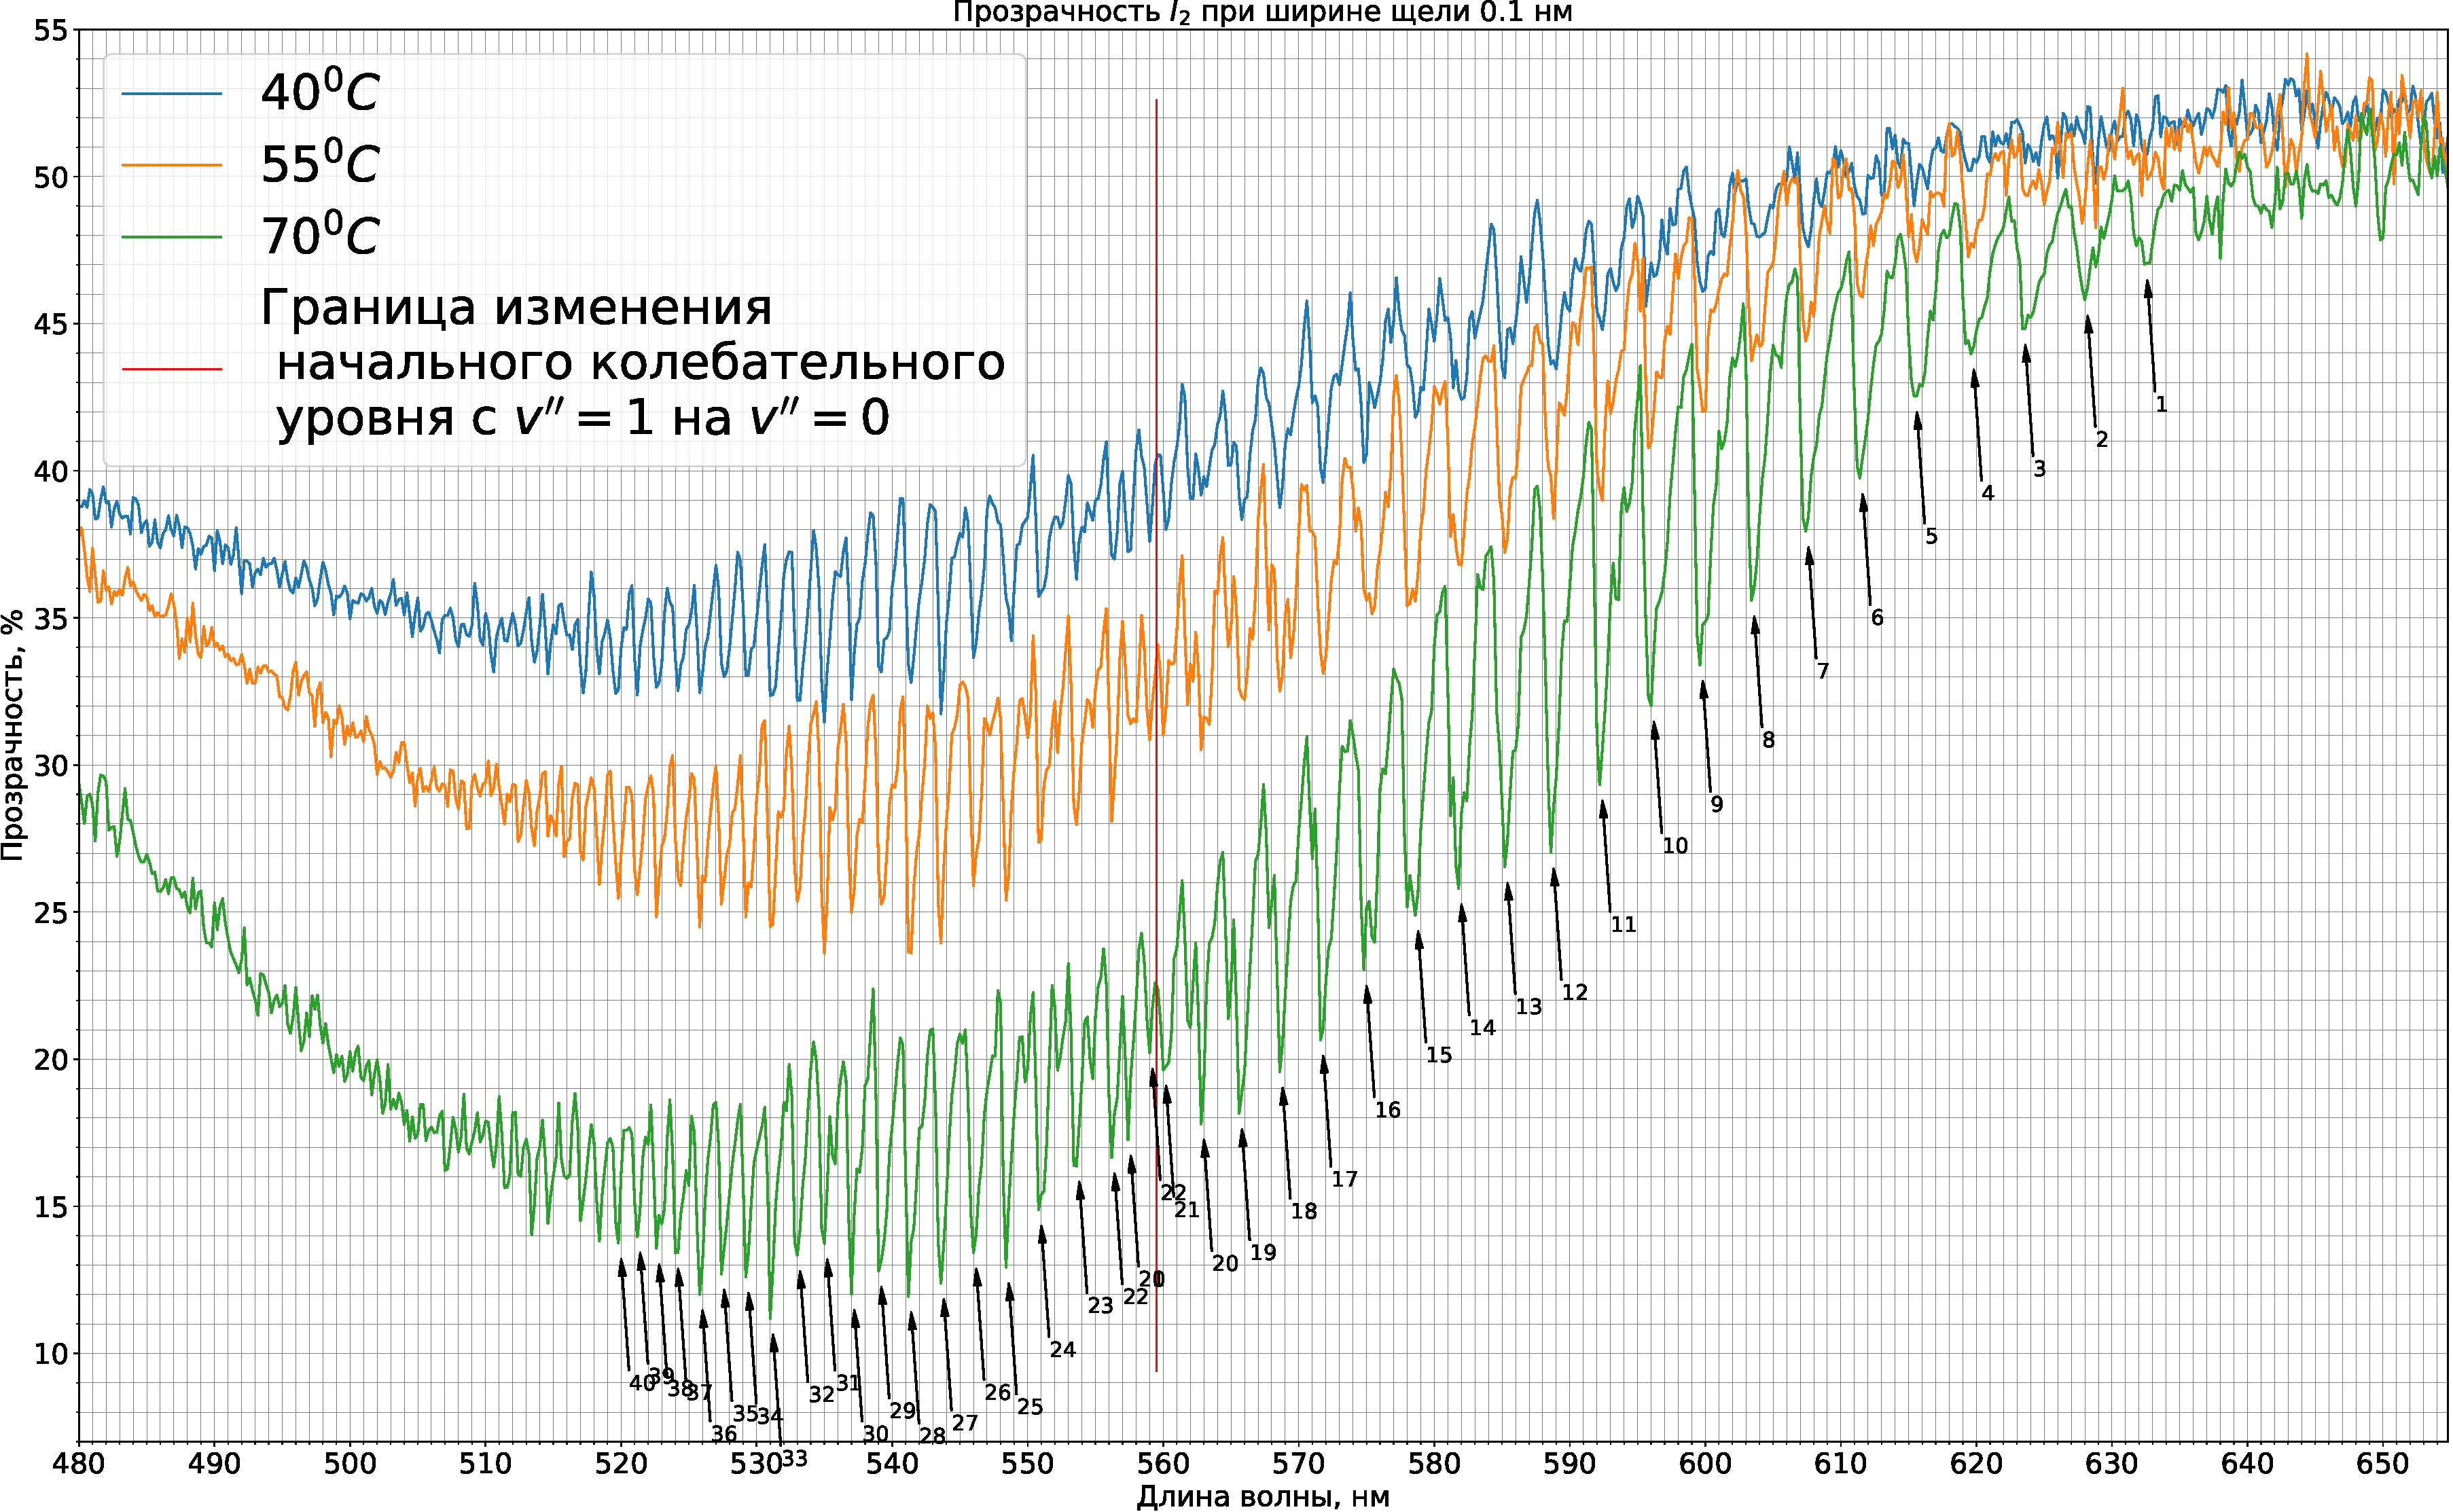
\includegraphics[angle = 90,
	% Высоту не менять! Подогнана)))
	height=0.88\textheight]{data/main_spectrum}
	\caption{Спектр поглощения молекулы I$_2$}
	\label{main_spectrum}
\end{figure}
\newpage
Видим, что при повышении температуры переходы становятся более отчетливыми, а прозрачность уменьшается. 

По спектру при температуре 70 $^\circ C$ составим таблицу \ref{tab:delandr} Деландра.

\begin{longtable}[h!]{|p{1cm}|p{3cm}|p{3cm}|}
	\caption{Таблица Деландра}\label{tab:delandr}\\
	\hline
	v'\textbackslash{}v'' & 0, см$^{-1}$ & 1, см $^{-1}$ \bigstrut\\
	\hline
	\endfirsthead
	\multicolumn{3}{p{8cm}}%
	{\tablename\ \thetable\ -- \textit{Продолжение с предыдущей страницы}} \\
	\hline
	v'\textbackslash{}v'' & 0, см$^{-1}$ & 1, см$^{-1}$ \bigstrut\\
	\hline
	\endhead
	\hline \multicolumn{3}{p{8cm}}{\textit{Продолжение на следующей странице}} \\
	\endfoot
	\hline
	\endlastfoot
	\hline
	1 &   & 15708 \bigstrut\\
	\hline
	2 &   & 15813 \bigstrut\\
	\hline
	3 &   & 15924 \bigstrut\\
	\hline
	4 &   & 16041 \bigstrut\\
	\hline
	5 &   & 16139 \bigstrut\\
	\hline
	6 &   & 16250 \bigstrut\\
	\hline
	7 &   & 16356 \bigstrut\\
	\hline
	8 &   & 16464 \bigstrut\\
	\hline
	9 &   & 16573 \bigstrut\\
	\hline
	10 &   & 16678 \bigstrut\\
	\hline
	11 &   & 16779 \bigstrut\\
	\hline
	12 &   & 16886 \bigstrut\\
	\hline
	13 &   & 16989 \bigstrut\\
	\hline
	14 &   & 17088 \bigstrut\\
	\hline
	15 &   & 17188 \bigstrut\\
	\hline
	16 &   & 17283 \bigstrut\\
	\hline
	17 &   & 17397 \bigstrut\\
	\hline
	18 &   & 17495 \bigstrut\\
	\hline
	19 &   & 17587 \bigstrut\\
	\hline
	20 & 17889 & 17680 \bigstrut\\
	\hline
	21 & 17979 & 17768 \bigstrut\\
	\hline
	22 & 18064 & 17857 \bigstrut\\
	\hline
	23 & 18155 &  \bigstrut\\
	\hline
	24 & 18235 &  \bigstrut\\
	\hline
	25 & 18315 &  \bigstrut\\
	\hline
	26 & 18396 &  \bigstrut\\
	\hline
	27 & 18477 &  \bigstrut\\
	\hline
	28 & 18553 &  \bigstrut\\
	\hline
	29 & 18622 &  \bigstrut\\
	\hline
	30 & 18692 &  \bigstrut\\
	\hline
	31 & 18762 &  \bigstrut\\
	\hline
	32 & 18832 &  \bigstrut\\
	\hline
	33 & 18896 &  \bigstrut\\
	\hline
	34 & 18961 &  \bigstrut\\
	\hline
	35 & 19019 &  \bigstrut\\
	\hline
	36 & 19084 &  \bigstrut\\
	\hline
	37 & 19135 &  \bigstrut\\
	\hline
	38 & 19186 &  \bigstrut\\
	\hline
	39 & 19238 &  \bigstrut\\
	\hline
	40 & 19290 &  \bigstrut\\
	\hline
\end{longtable}
\subsection{Линейная аппроксимация}
Вычислим разности соседних волновых чисел в полученных $v'$-прогрессиях \\$\nu(v'+1)-\nu(v')= \Delta G'_{v'+0.5}$. Используя полученные значения, проведем регрессионный анализ зависимости $\Delta G'_{v'+0.5}(v'+1)$ при $v'' = 0; 1$ (рис. \ref{deltaG0}, \ref{deltaG1}).

\begin{figure}[h!]
	\centering
	\includegraphics[width=0.81\linewidth]{data/deltaG(v_0).pdf}
	\caption{Линейная аппроксимация ($v''=0$)}
	\label{deltaG0}
\end{figure}
\begin{figure}[h!]
	\centering
	\includegraphics[width=0.79\linewidth]{data/deltaG(v_1).pdf}
	\caption{Линейная аппроксимация ($v''=1$)}
	\label{deltaG1}
\end{figure}

Отсюда, получаем результат (табл. \ref{tab:linear_approx}).
% Table generated by Excel2LaTeX from sheet 'Пункт 3'
\begin{table}[h!]
	\centering
	\caption{Результаты линейной аппроксимации}
	\begin{tabular}{|c|c|c|c|}
		\hline
		\multicolumn{1}{|l|}{v''} & \multicolumn{1}{l|}{$\omega_e'$, см$^{-1}$} & \multicolumn{1}{l|}{$\omega_e' x_e'$, см$^{-1}$} & \multicolumn{1}{c|}{$\rho$} \bigstrut\\
		\hline
		0 & $133\pm 3$ & $1.07\pm 0.05$& -0.95 \bigstrut\\
		\hline
		1 & $114\pm 3$& $0.53\pm 0.13$ & -0.75 \bigstrut\\
		\hline
	\end{tabular}%
	\label{tab:linear_approx}%
\end{table}%

\subsection{Определение молекулярных констант методом параболического регрессионного анализа}

Определим значение $\omega'_e$, $\omega'_e x_e'$, а также величину электронного терма $T_e$ возбужденного состояния $^3\Pi^+_{0u}$, используя зависимость \eqref{wave_counts}:
\begin{equation}
\nu = \nu_{\text{эл}} + \left[\omega'_e\left(v'+\frac{1}{2}\right)-\omega'_e x_e'\left(v'+\frac{1}{2}\right)^2\right]-\left[\omega''_e\left(v''+\frac{1}{2}\right)-\omega''_e x_e''\left(v''+\frac{1}{2}\right)^2\right].
\label{wave_counts}
\end{equation}
Применяя метод параболического регрессионного анализа для выделенных $v'$ прогрессий, получим рис. \ref{parabola_half_0}, \ref{parabola_half_1}, а численный результат занесем в таблицу \ref{tab:parabola}.
\begin{figure}[h!]
	\centering
	\includegraphics[height=0.4\textheight]{data/parabola_half_0}
	\caption{Параболическая аппроксимация ($v'' = 0$)}
	\label{parabola_half_0}
\end{figure}
\begin{figure}[h!]
	\centering
	\includegraphics[height=0.4\textheight]{data/parabola_half_1}
	\caption{Параболическая аппроксимация ($v'' = 1$)}
	\label{parabola_half_1}
\end{figure}

% Table generated by Excel2LaTeX from sheet '4 пункт'
\begin{table}[htbp]
	\centering
	\caption{Результаты анализа для выделенных $v'$ прогрессий}
	\begin{tabular}{|r|r|r|r|}
		\hline
		\multicolumn{1}{|l|}{v''} & \multicolumn{1}{l|}{$T_e$, см$^{-1}$} & \multicolumn{1}{l|}{$\omega'_e$, см$^{-1}$} & \multicolumn{1}{l|}{$\omega'_e x'_e$, см$^{-1}$} \bigstrut\\
		\hline
		0 & 15765 & 132.9 & 1.063 \bigstrut\\
		\hline
		1 & 15793 & 125.9 & 0.54 \bigstrut\\
		\hline
	\end{tabular}%
	\label{tab:parabola}%
\end{table}%

Вычислим волновое число $\nu_{0,0} \cong T_e + 0.5\omega_e' - 0.5\omega_e''$ ($\omega_e''$ для $I_2$ равна $214$ см$^{-1}$)
\begin{equation}
\nu_{0,0} = 15750 \text{ см$^{-1}$}
\end{equation}


\subsection{Вычисление $\nu_{\text{гр}}$}
По экспериментальным значениям волновых чисел $\nu_{0,v'}$ для переходов $v''= 0 \to v'$ определим волновое число границы непрерывного спектра поглощения $\nu_{\text{гр}}$ , считая, что волновые числа полос $\nu(v')$ и их разности $\Delta \nu =\nu(v'+1)-\nu(v')$ связаны квадратичной зависимостью
вида \eqref{delta_nu}.
\begin{equation}
\nu = \nu_{\text{гр}} +b\Delta\nu+c\left(\Delta \nu\right)^2
\label{delta_nu}
\end{equation}
Результат аппроксимации параболой представлен на рис. \ref{fig:delta_nu}, а численное значение $\nu_{\text{гр}}$ есть
\begin{equation}
\nu_{\text{гр}} = (19.9 \pm 0.6) \cdot 10^3 \text{ см$^{-1}$}
\end{equation}
\begin{figure}[h!]
	\centering
	\includegraphics[height=0.45\textheight]{data/delta_nu}
	\caption{Определение границы сплошного спектра}
	\label{fig:delta_nu}
\end{figure}

\subsection{Определение энергий диссоциации}
Используя полученные ранее значения молекулярных постоянных, определим энергию диссоциации $D_0'$ для возбужденного электронного состояния $^3\Pi^+_{0u}$ тремя способами:
\begin{enumerate}
	\item По формуле линейной экстраполяции 
	\begin{equation}
	D_0'=\cfrac{\omega_e'^2}{4\omega_e'x_e'} = 4133 \text{ см$^{-1}$}
	\end{equation}
	\item По границе сплошного спектра
	\begin{equation}
	D_0'=\nu_{\text{гр}}- \nu_{00} = 4150 \text{ см$^{-1}$}
	\end{equation}
	\item Методом Берджа-Шпонер
\end{enumerate}
Для подсчета методом Берджа-Шпонер необходимо величины разностей $\Delta G'_{v'+0.5}$ отнести к серединам колебательных интервалов, т.е. к $v'+0.5$, а далее экстраполировать параболой (рис. \ref{fig:deltaG_half_berdg}). Площадь под этой кривой соответствует энергии диссоциации.
\begin{figure}[h!]
	\centering
	\includegraphics[height=0.45\textheight]{data/deltaG_half_berdg}
	\caption{Экстраполяция методом Берджа-Шпонер}
	\label{fig:deltaG_half_berdg}
\end{figure}
Проинтегрировав аппроксимацию, получим
\begin{equation}
D_0' = 3664 \text{ см$^{-1}$}
\end{equation}

Определим энергию диссоциации $D_0''$ для основного электронного состояния $^1\Sigma_g^{+}$ по границе сплошного спектра ($E_a = 7603$ см$^{-1}$)
\begin{equation}
D_0'' = \nu_{\text{гр}}-E_a = 12297 \text{ см$^{-1}$}
\end{equation}
\subsection{Определение межъядерного расстояния, построение потенциальной кривой Морзе}
Для прогрессии с $v'' = 0$ определим волновое число полосы с максимальным поглощением (у нас это пик под номером $33$)
\begin{equation}
\nu_{max}  = 18896 \text{ см$^{-1}$}
\end{equation}
Определим равновесное межъядерное положение $r_e'$ для возбужденного электронного состояния $^3\Pi^+_{0u}$, используя уравнения \eqref{eq:pot_en_r_e}, \eqref{eq:r_e'} и полученные из опыта значения $\nu_{max}, \omega_e', D_0'$. Примем, что $r_e'' = 2.67$ \AA.
\begin{equation}
\label{eq:pot_en_r_e}
U'(r'=r_e'') \cong \nu_{max} - \nu_{0,0}+\cfrac{\omega_e'}{2} = 3213 \text{ см}^{-1}
\end{equation}
\begin{equation}
\label{eq:r_e'}
r_e'=r_e'' + \frac{1}{\beta'}\,\ln\left[1+\left(\cfrac{U'(r'=r_e'')}{D_e'}\right)^{1/2}\right]
\end{equation}
где $D'_e \cong D'_0 + \dfrac{\omega'_e}{2} = 3731 \text{ см}^{-1},~ 
\beta' = \omega'_e \left( \dfrac{2 \pi^2 \mu c}{D'_e h} \right)^{1/2} 
\approx 0.12177 \omega'_e \sqrt{ \dfrac{\mu}{D'_e} }
\approx 4.23 \text{ см}^{-1}$, если $\omega'_e$, $D'_e$ выражены в см$^{-1}$, $\mu$ - в а.е.м.

После численных подстановок получим
\begin{equation}
r_e' = 2.825 \text{ \AA}
\end{equation}
Построим потенциальную кривую возбужденного электронного состояния $^3\Pi^+_{0u}$, используя функцию Морзе (рис. \ref{fig:morse}). Для этого найдем $D'_e = D'_0 + hc(\frac{1}{2}\omega'_e - \frac{1}{4}\omega'_e x'_e) = 4216 \text{см}^{-1} = 0.527 \text{эВ}$
\begin{figure}[h!]
	\centering
	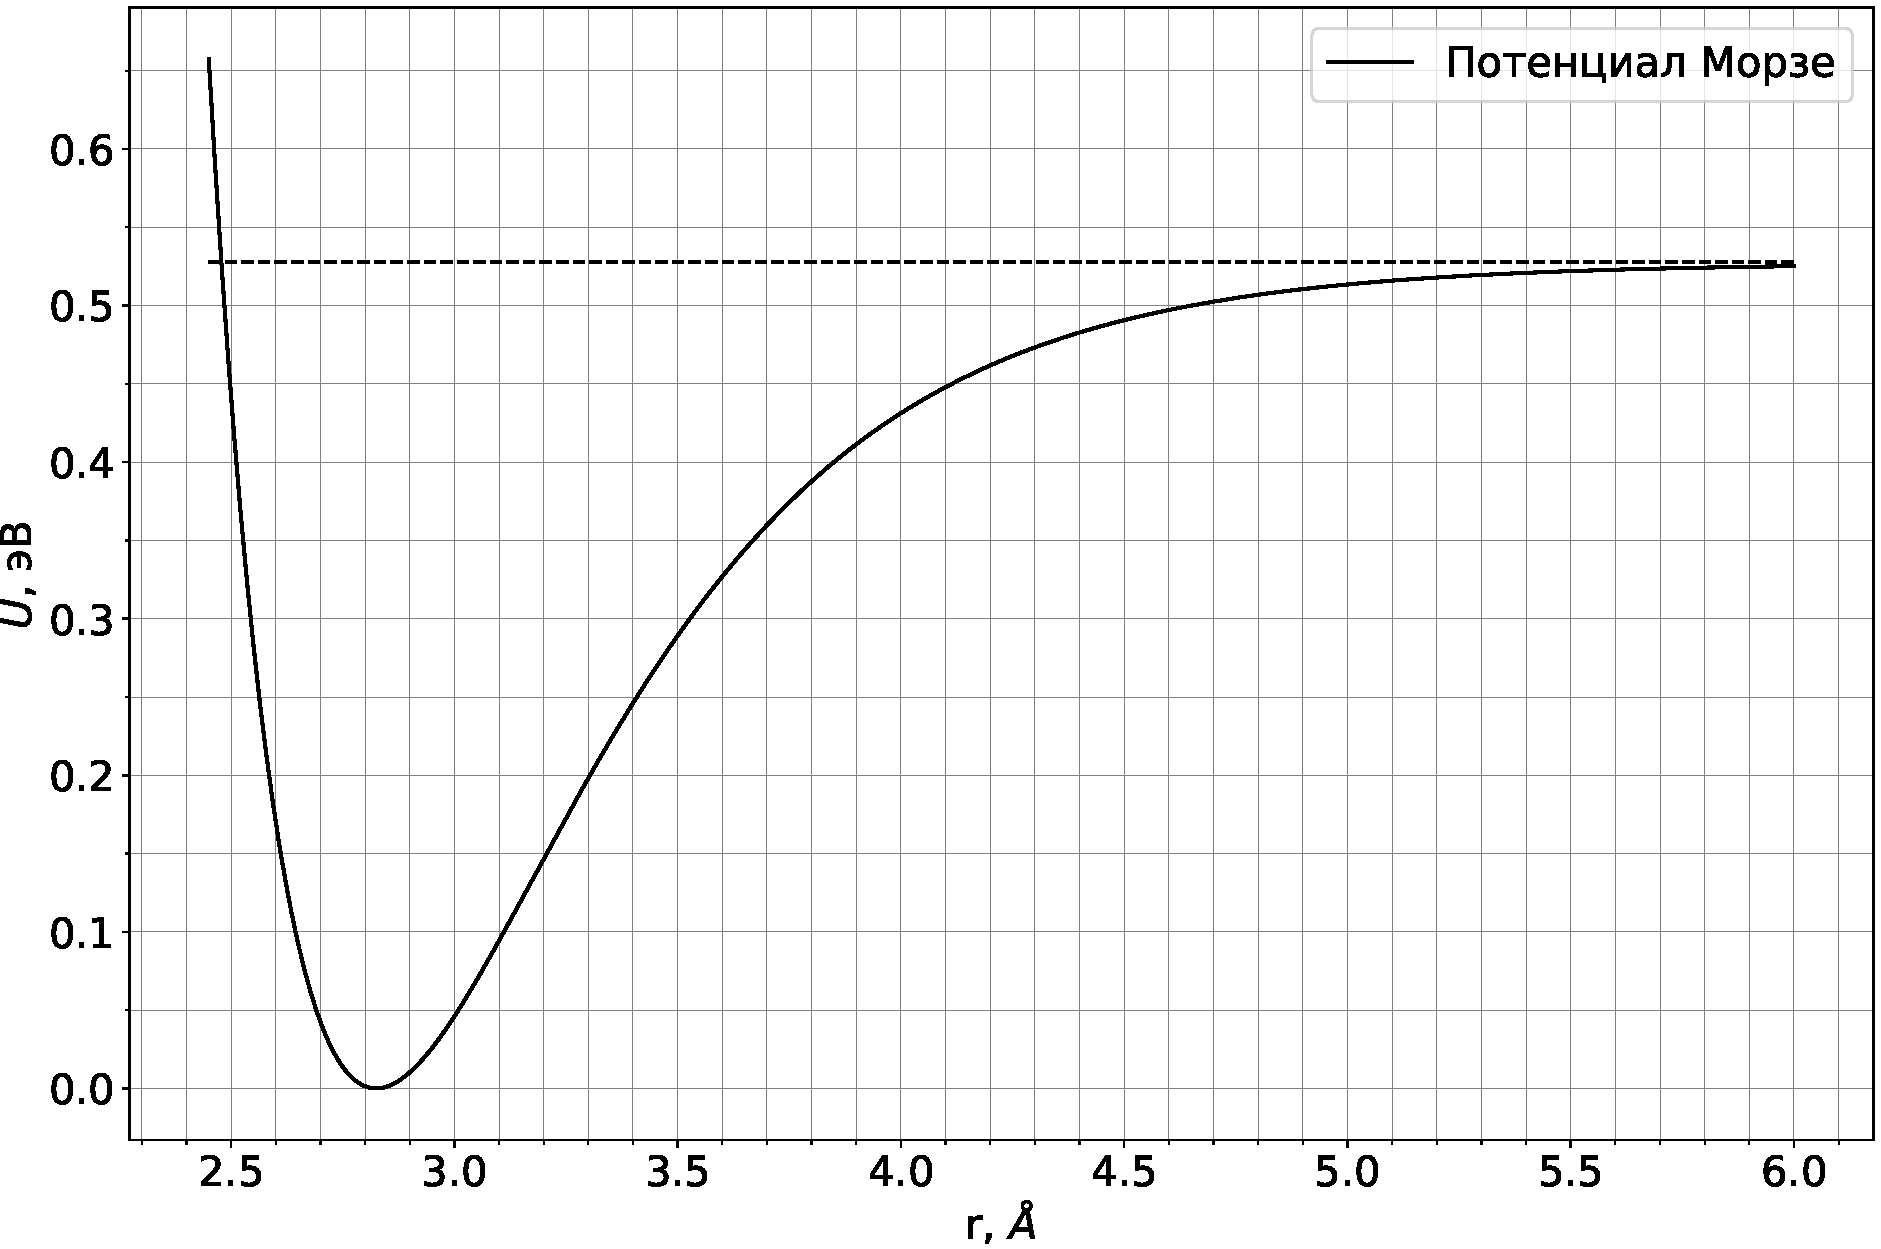
\includegraphics[height=0.45\textheight]{data/morse}
	\caption{Потенциал Морзе для электронного состояния $^3\Pi^+_{0u}$}
	\label{fig:morse}
\end{figure}

\subsection{Результат вычислений}
Все результаты занесем в таблицу \ref{table:final_results}.
% Table generated by Excel2LaTeX from sheet 'Результаты'
\begin{table}[h!]
	\centering
	\caption{Результаты определения молекулярных постоянных}
	\begin{tabular}{|c|c|c|c|c|c|c|}
		\hline
		$T_e$, см$^{-1}$ & $\omega_e'$, см$^{-1}$ & $\omega_e'x_e'$, см$^{-1}$ & $r_e'$, \AA & Энергия диссоциации & $D_0'$, см$^{-1}$; эВ & $D_0''$, см$^{-1}$; эВ \bigstrut\\
		\hline
		\multirow{3}[6]{*}{15765} & \multirow{3}[6]{*}{133} & \multirow{3}[6]{*}{1.07} & \multirow{3}[6]{*}{2.972} & \makecell{По границе \\сплошного спектра} & 4150; 0.513 & 12297; 1.529 \bigstrut\\
		\cline{5-7}       &   &   &   & \makecell{Экстраполяция \\Берджа--Шпонер} & 3664; 0.455 &  \bigstrut\\
		\cline{5-7}       &   &   &   & \makecell{Линейная \\экстраполяция} & 4133; 0.514 &  \bigstrut\\
		\hline
		\multicolumn{7}{|c|}{Табличные данные} \bigstrut\\
		\hline
		15770.6& 125.3  & 0.702  &  3.028 &   & 4320; 0.536  & 12440; 1.542 \bigstrut\\
		\hline
		
	\end{tabular}%
	\label{table:final_results}%
\end{table}%

\subsection{Сравнение спектров при разных ширинах щели}
Проведем сравнение спектров, зарегистрированных при разных ширинах щели (рис. \ref{fig:absorption_spectrum_slit}).
\begin{figure}[H]
	\begin{minipage}[h]{0.5\linewidth}
		\centering
		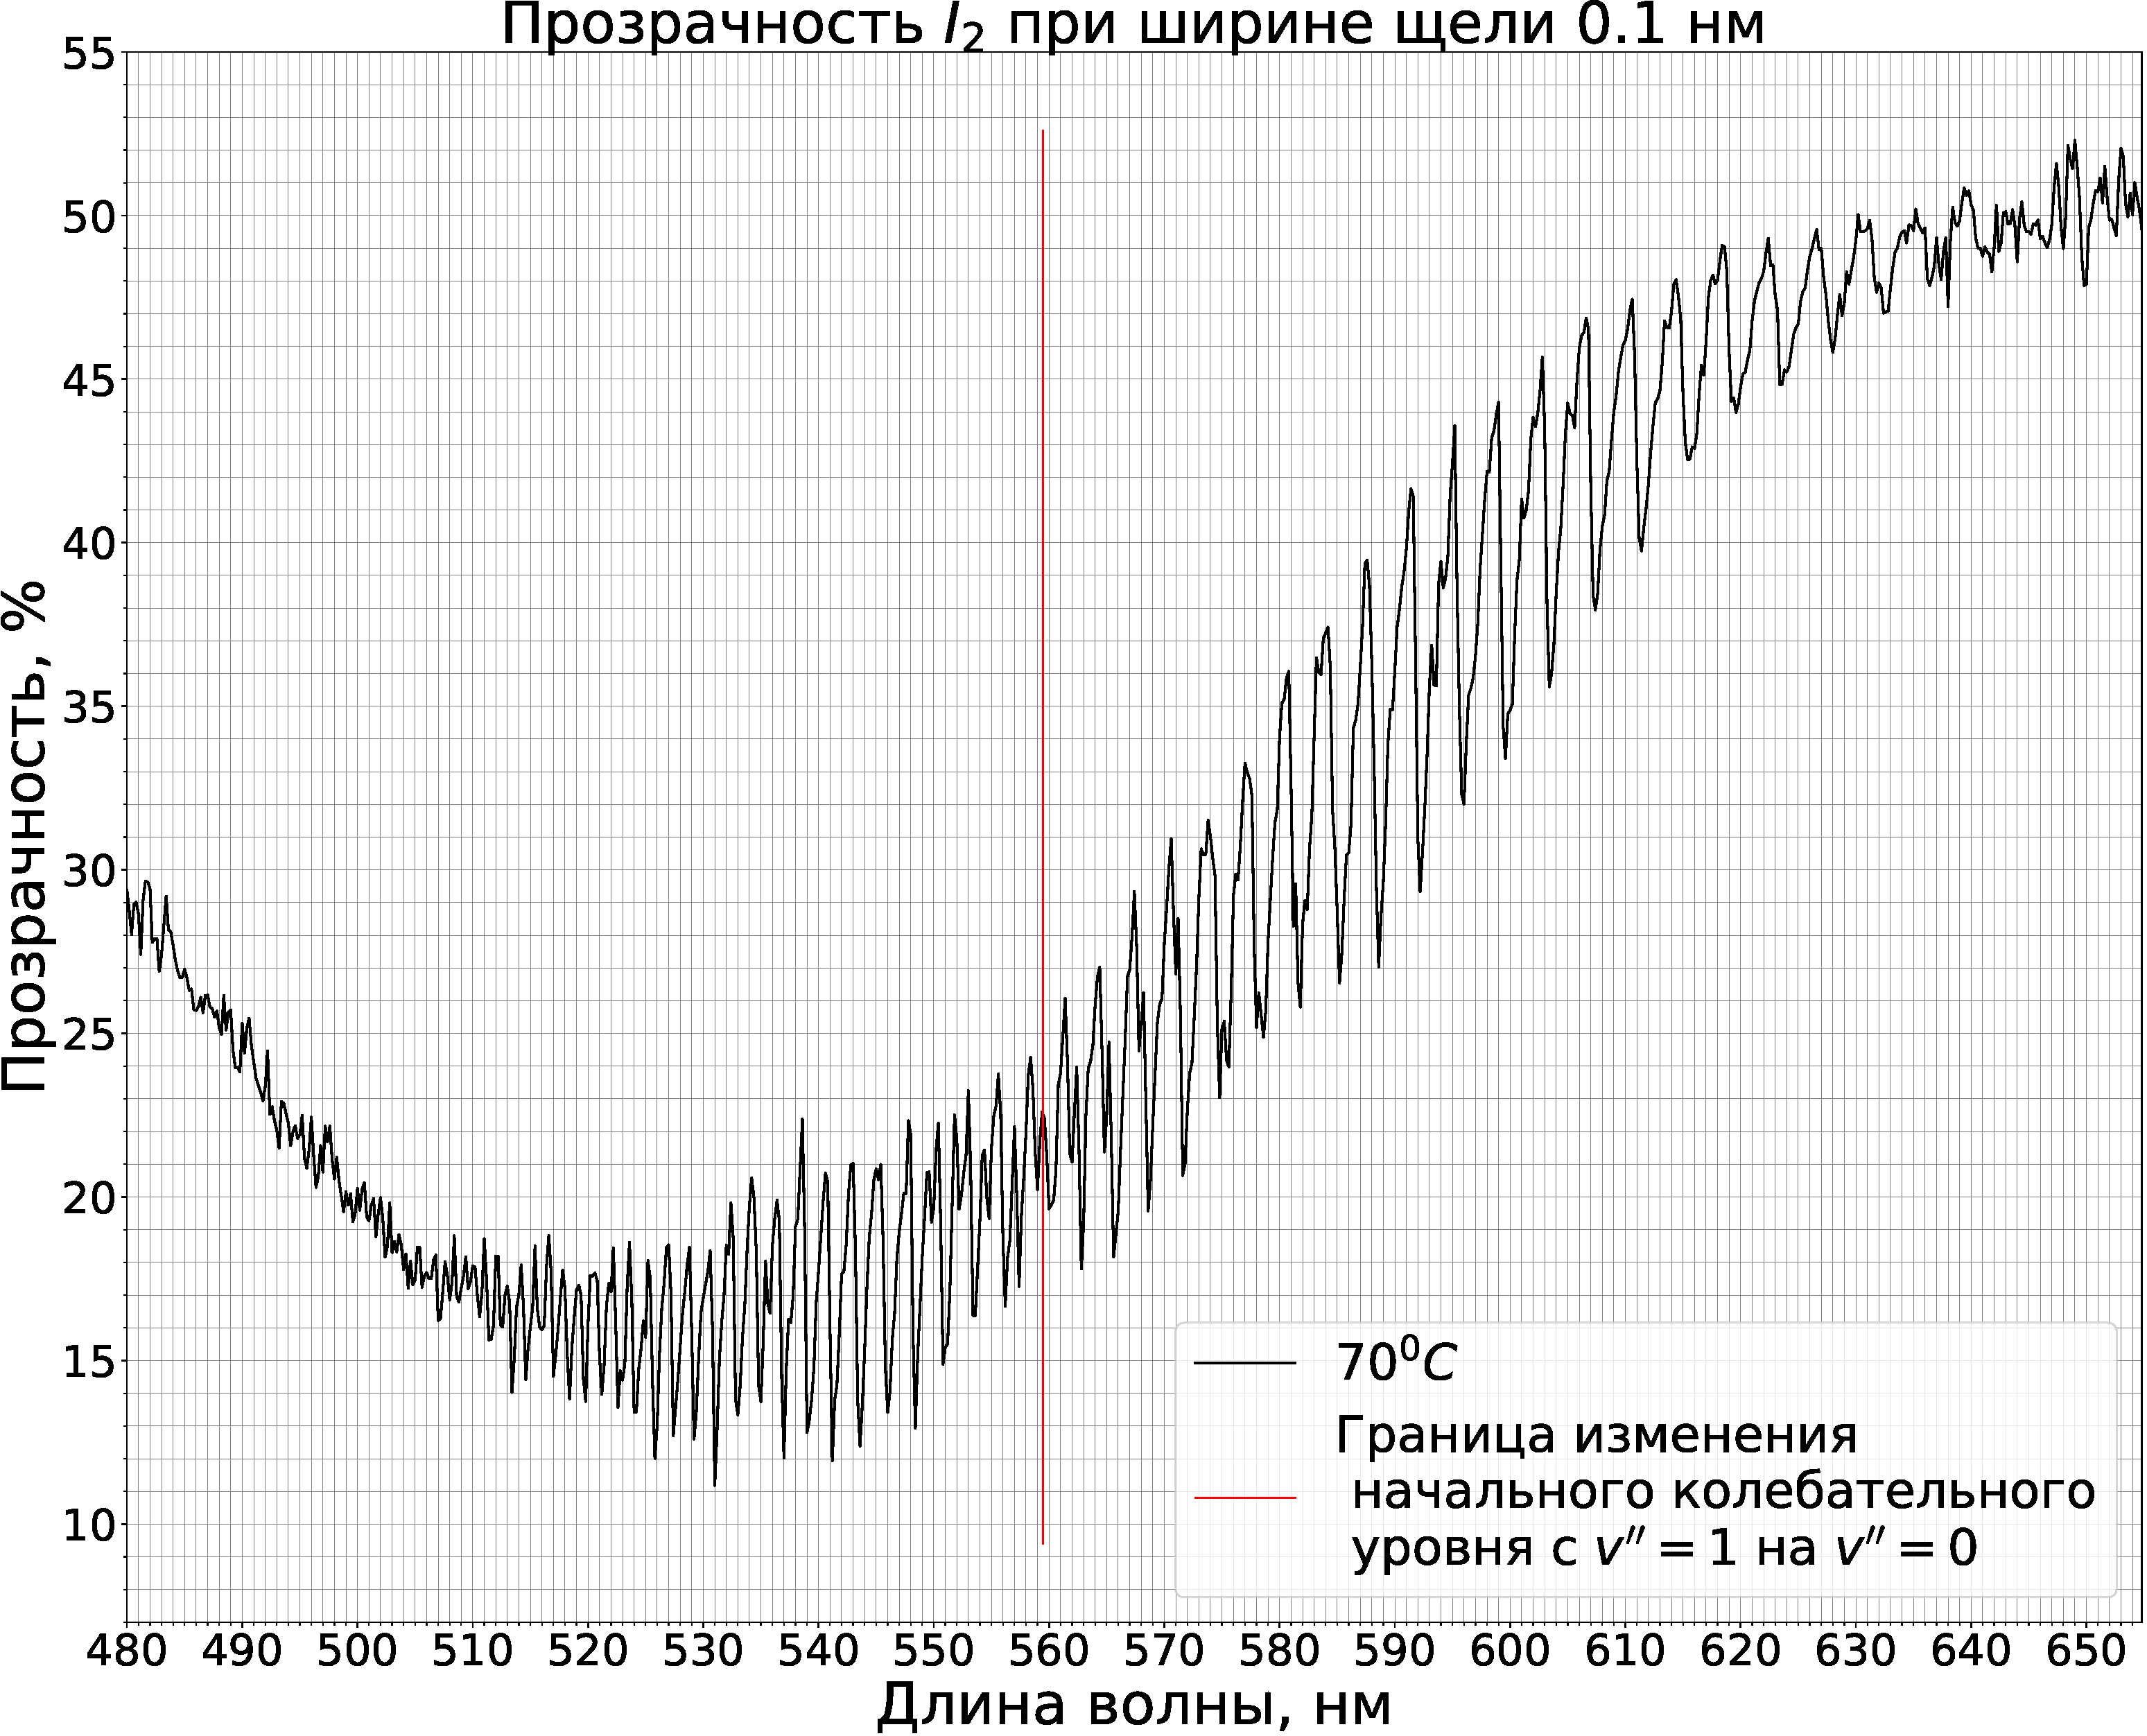
\includegraphics[width=1\linewidth]{data/absorption_spectrum_slit_01}
	\end{minipage}
	\begin{minipage}[h!]{0.5\linewidth}
		\centering
		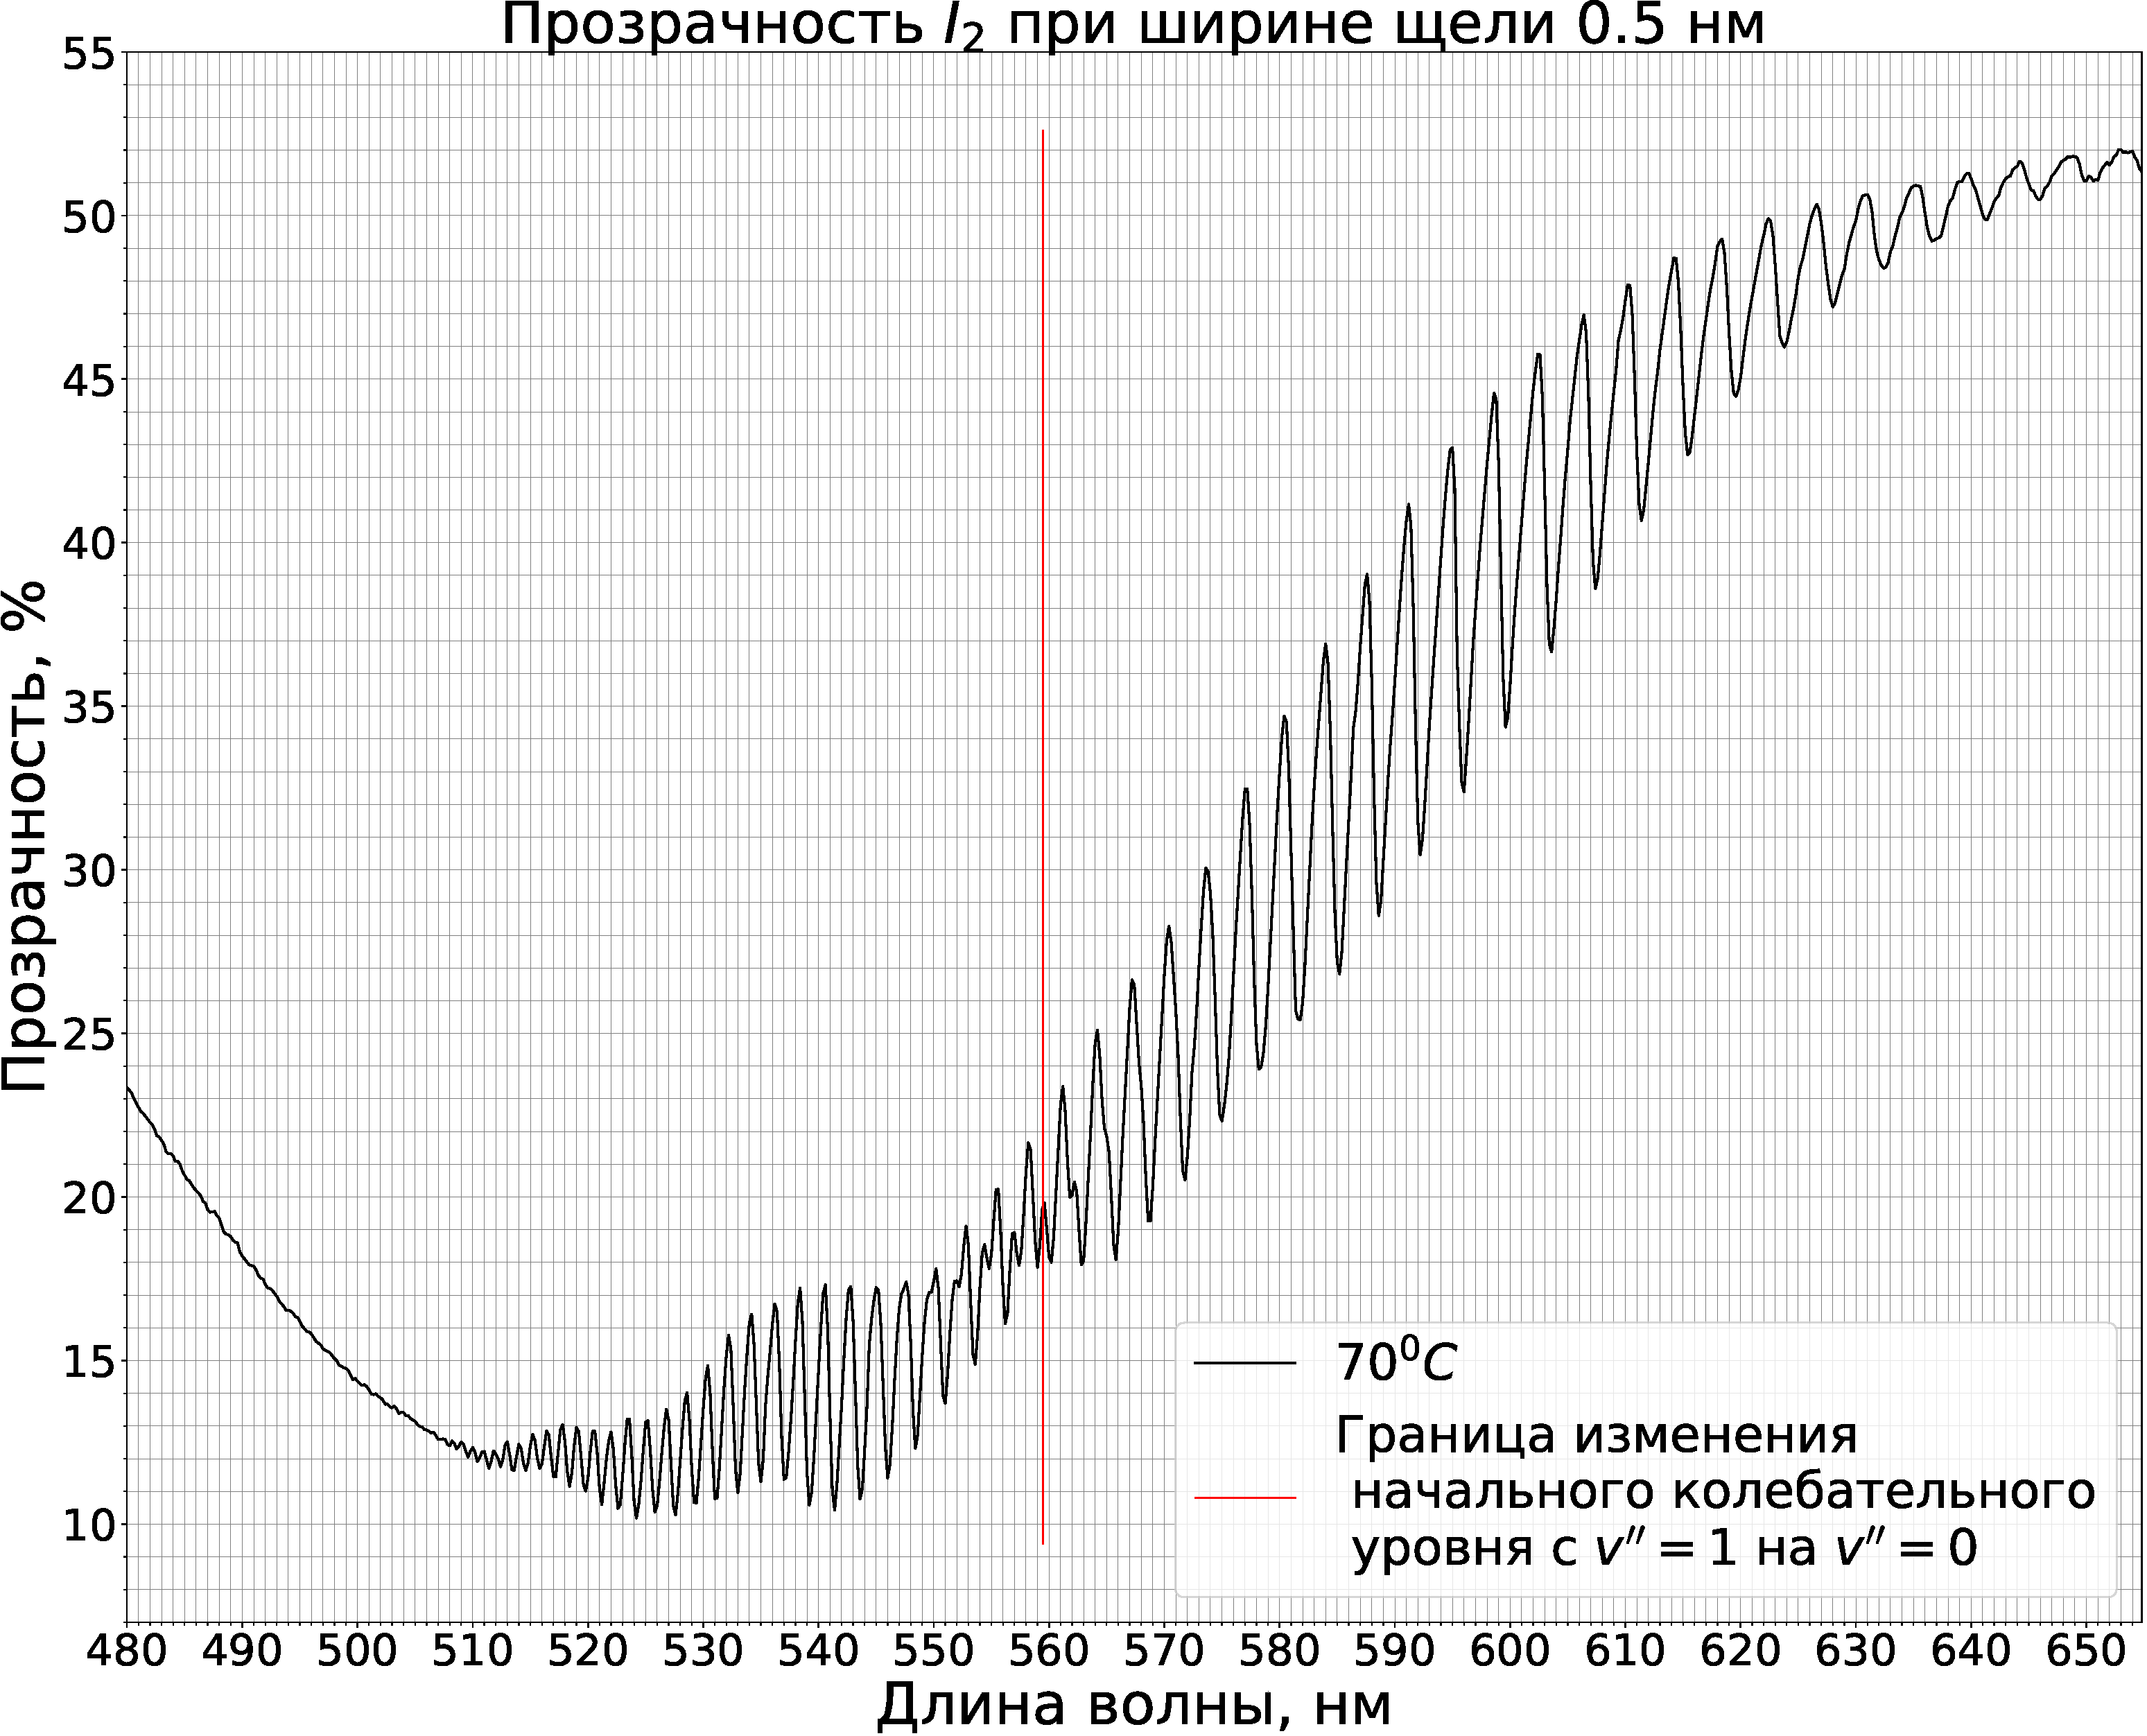
\includegraphics[width=1\linewidth]{data/absorption_spectrum_slit_05}
	\end{minipage}
	\begin{minipage}[h!]{0.5\linewidth}
		\centering
		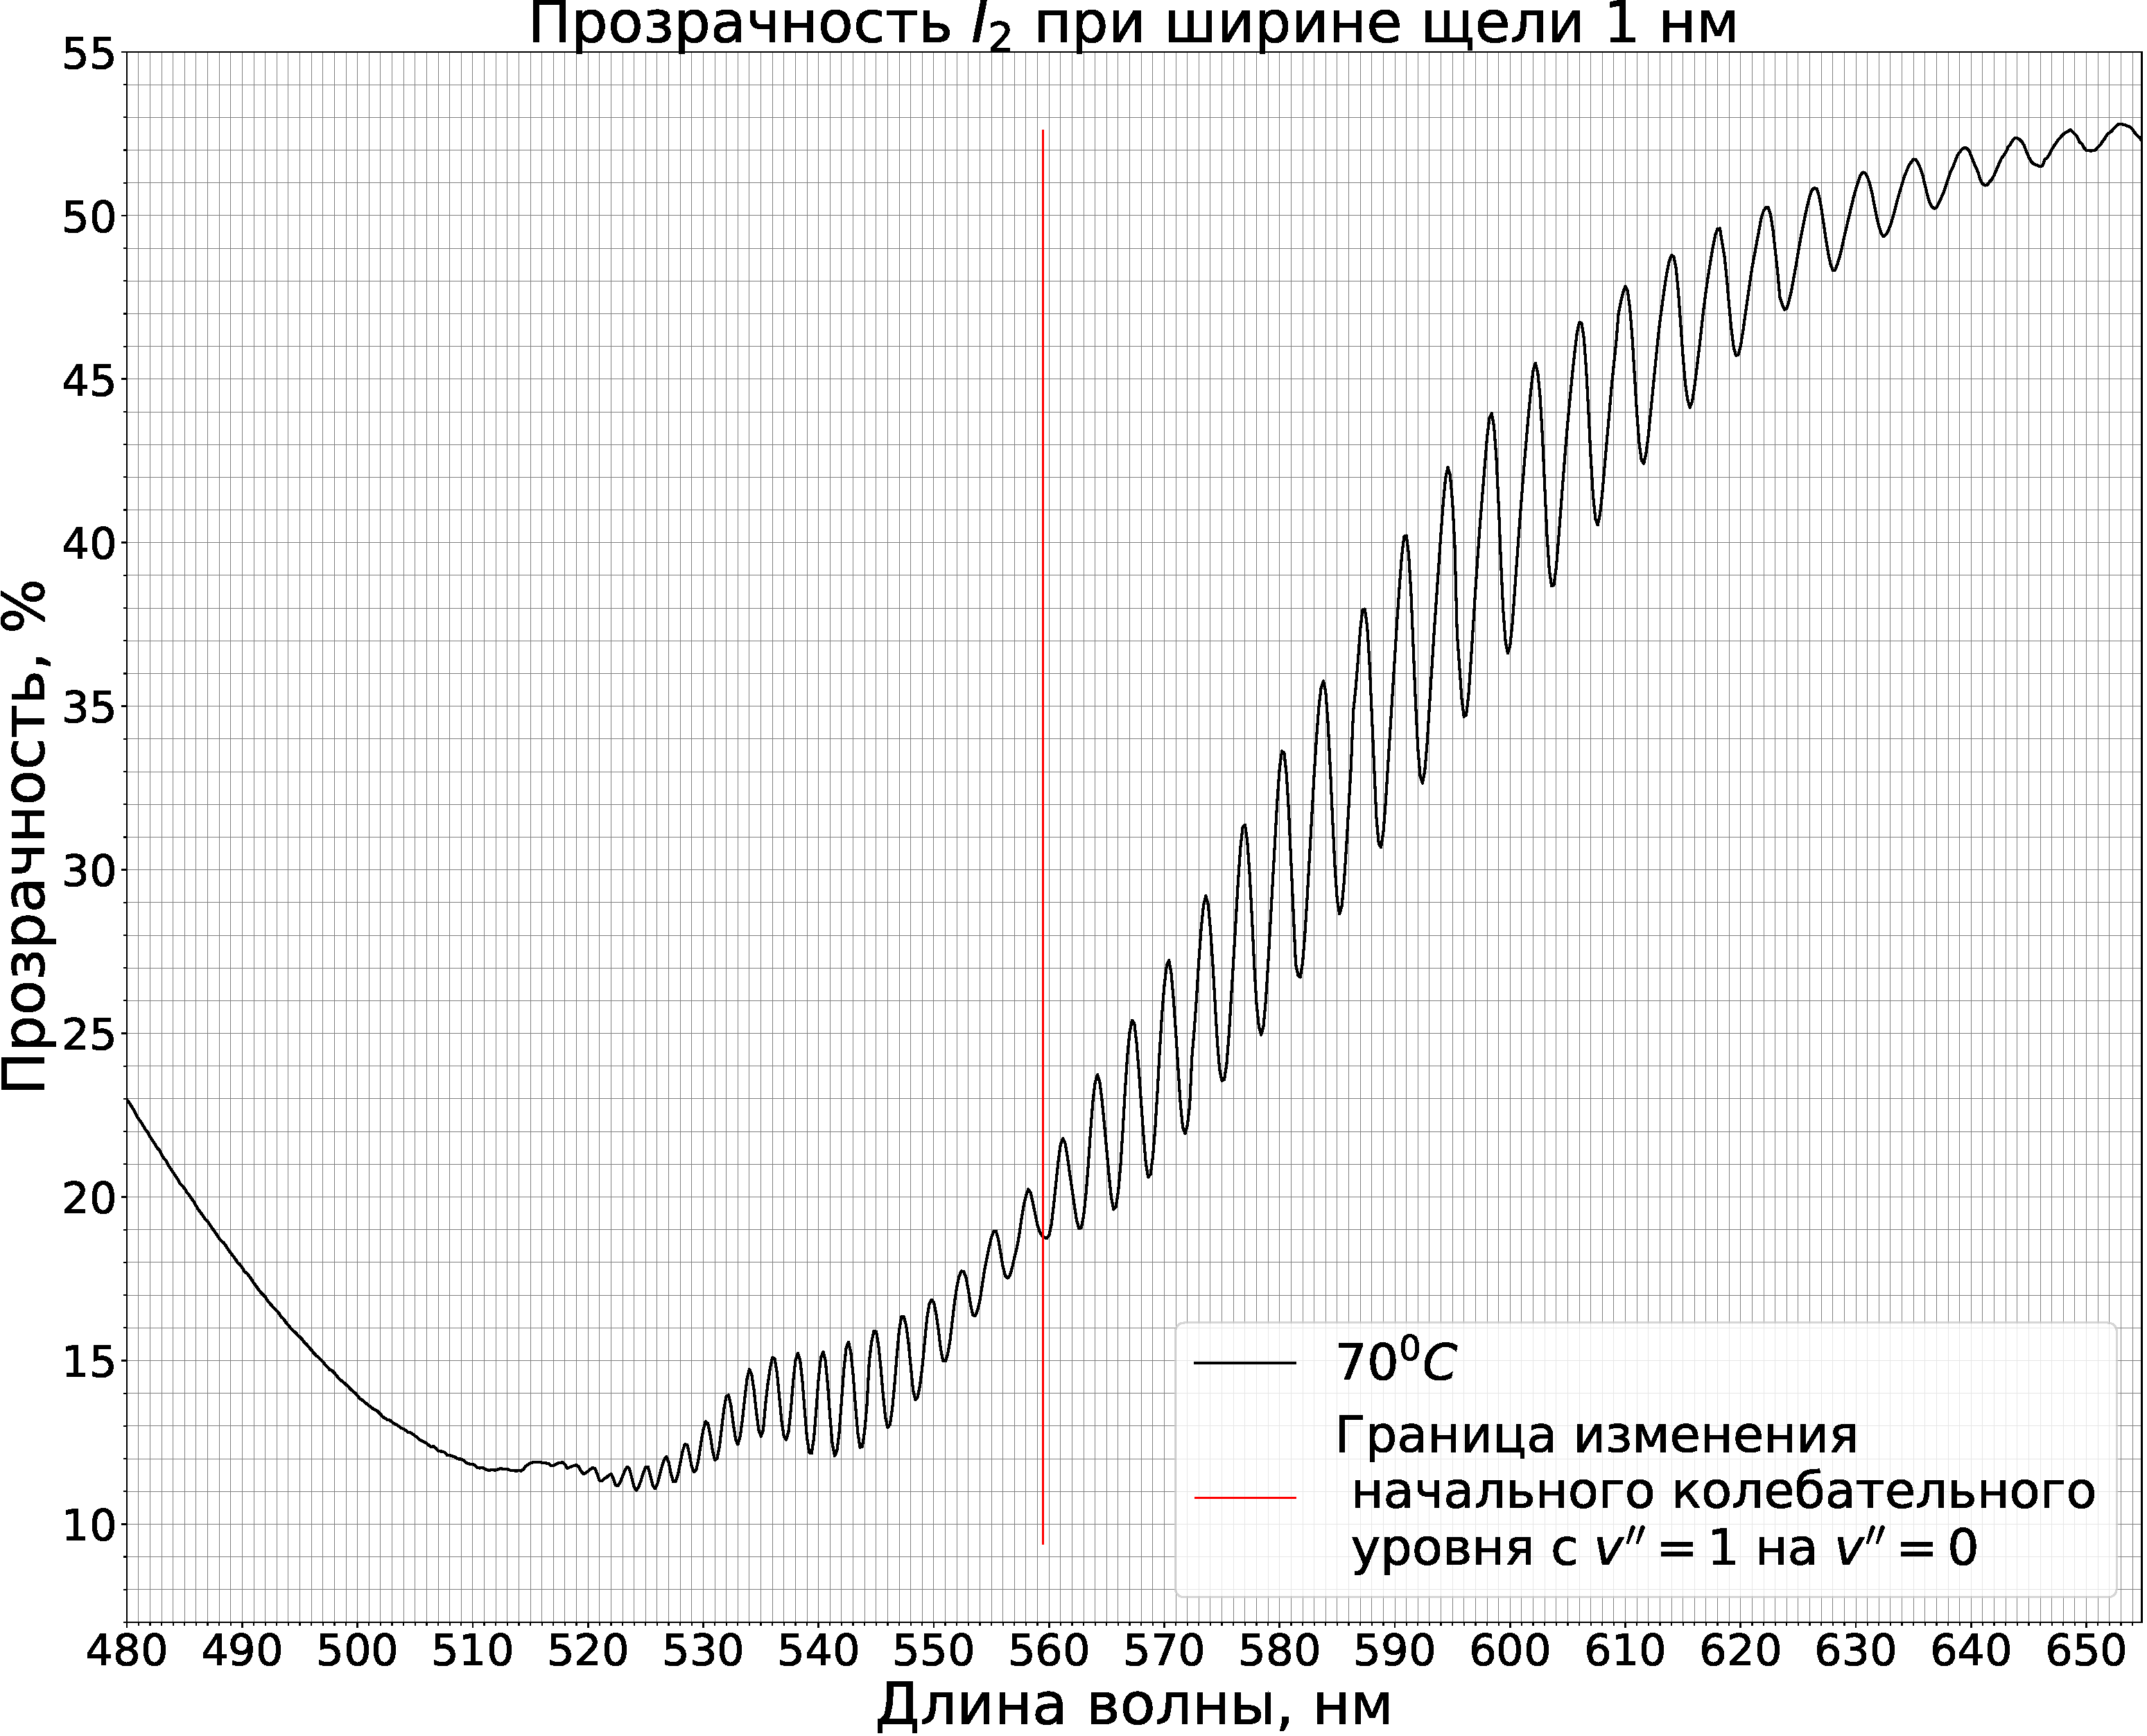
\includegraphics[width=1\linewidth]{data/absorption_spectrum_slit_1}
	\end{minipage}
	\begin{minipage}[h!]{0.5\linewidth}
		\centering
		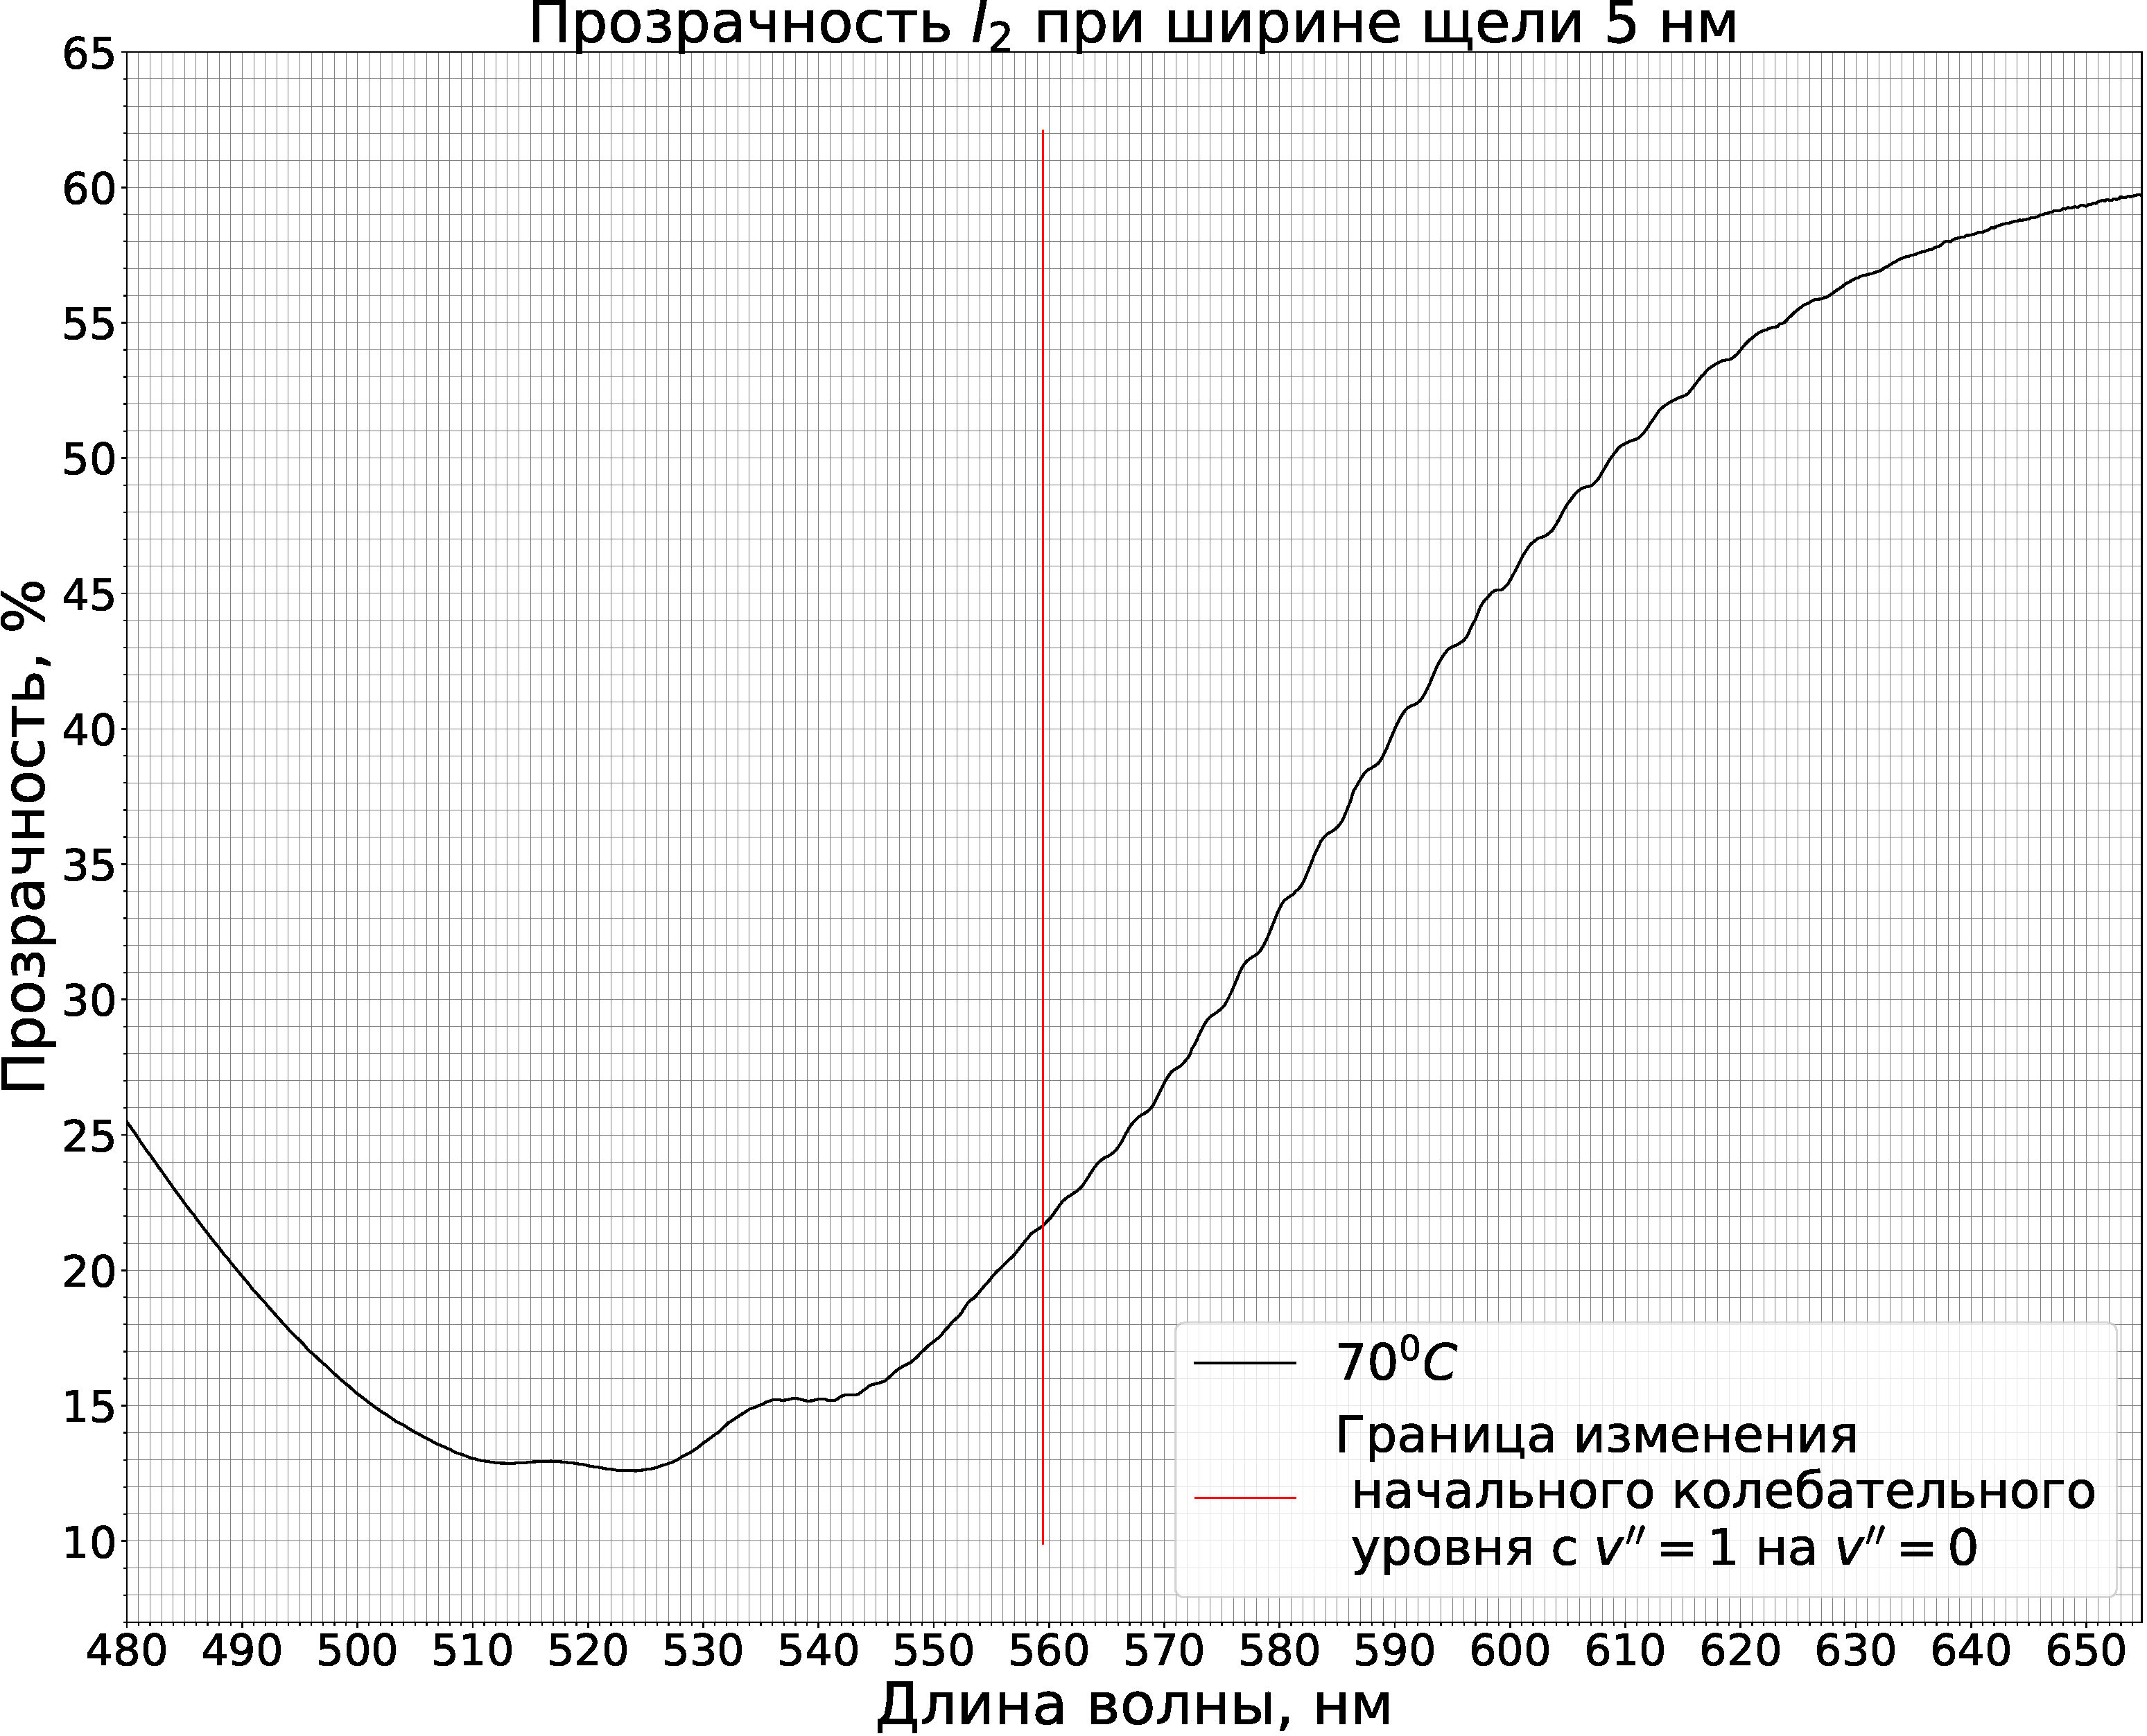
\includegraphics[width=1\linewidth]{data/absorption_spectrum_slit_5}
	\end{minipage}
	\caption{Вид спектра при различных ширинах щели}
	\label{fig:absorption_spectrum_slit}
\end{figure}
Видим, что чем больше размер щели, тем меньшее различие в энергии мы способны различить.

\subsection{Спектр широкого диапазона}
Рассмотрим спектр для диапазона длин волн 330--700 нм (рис. \ref{long_spectrum}).
\begin{figure}[H]
	\centering
	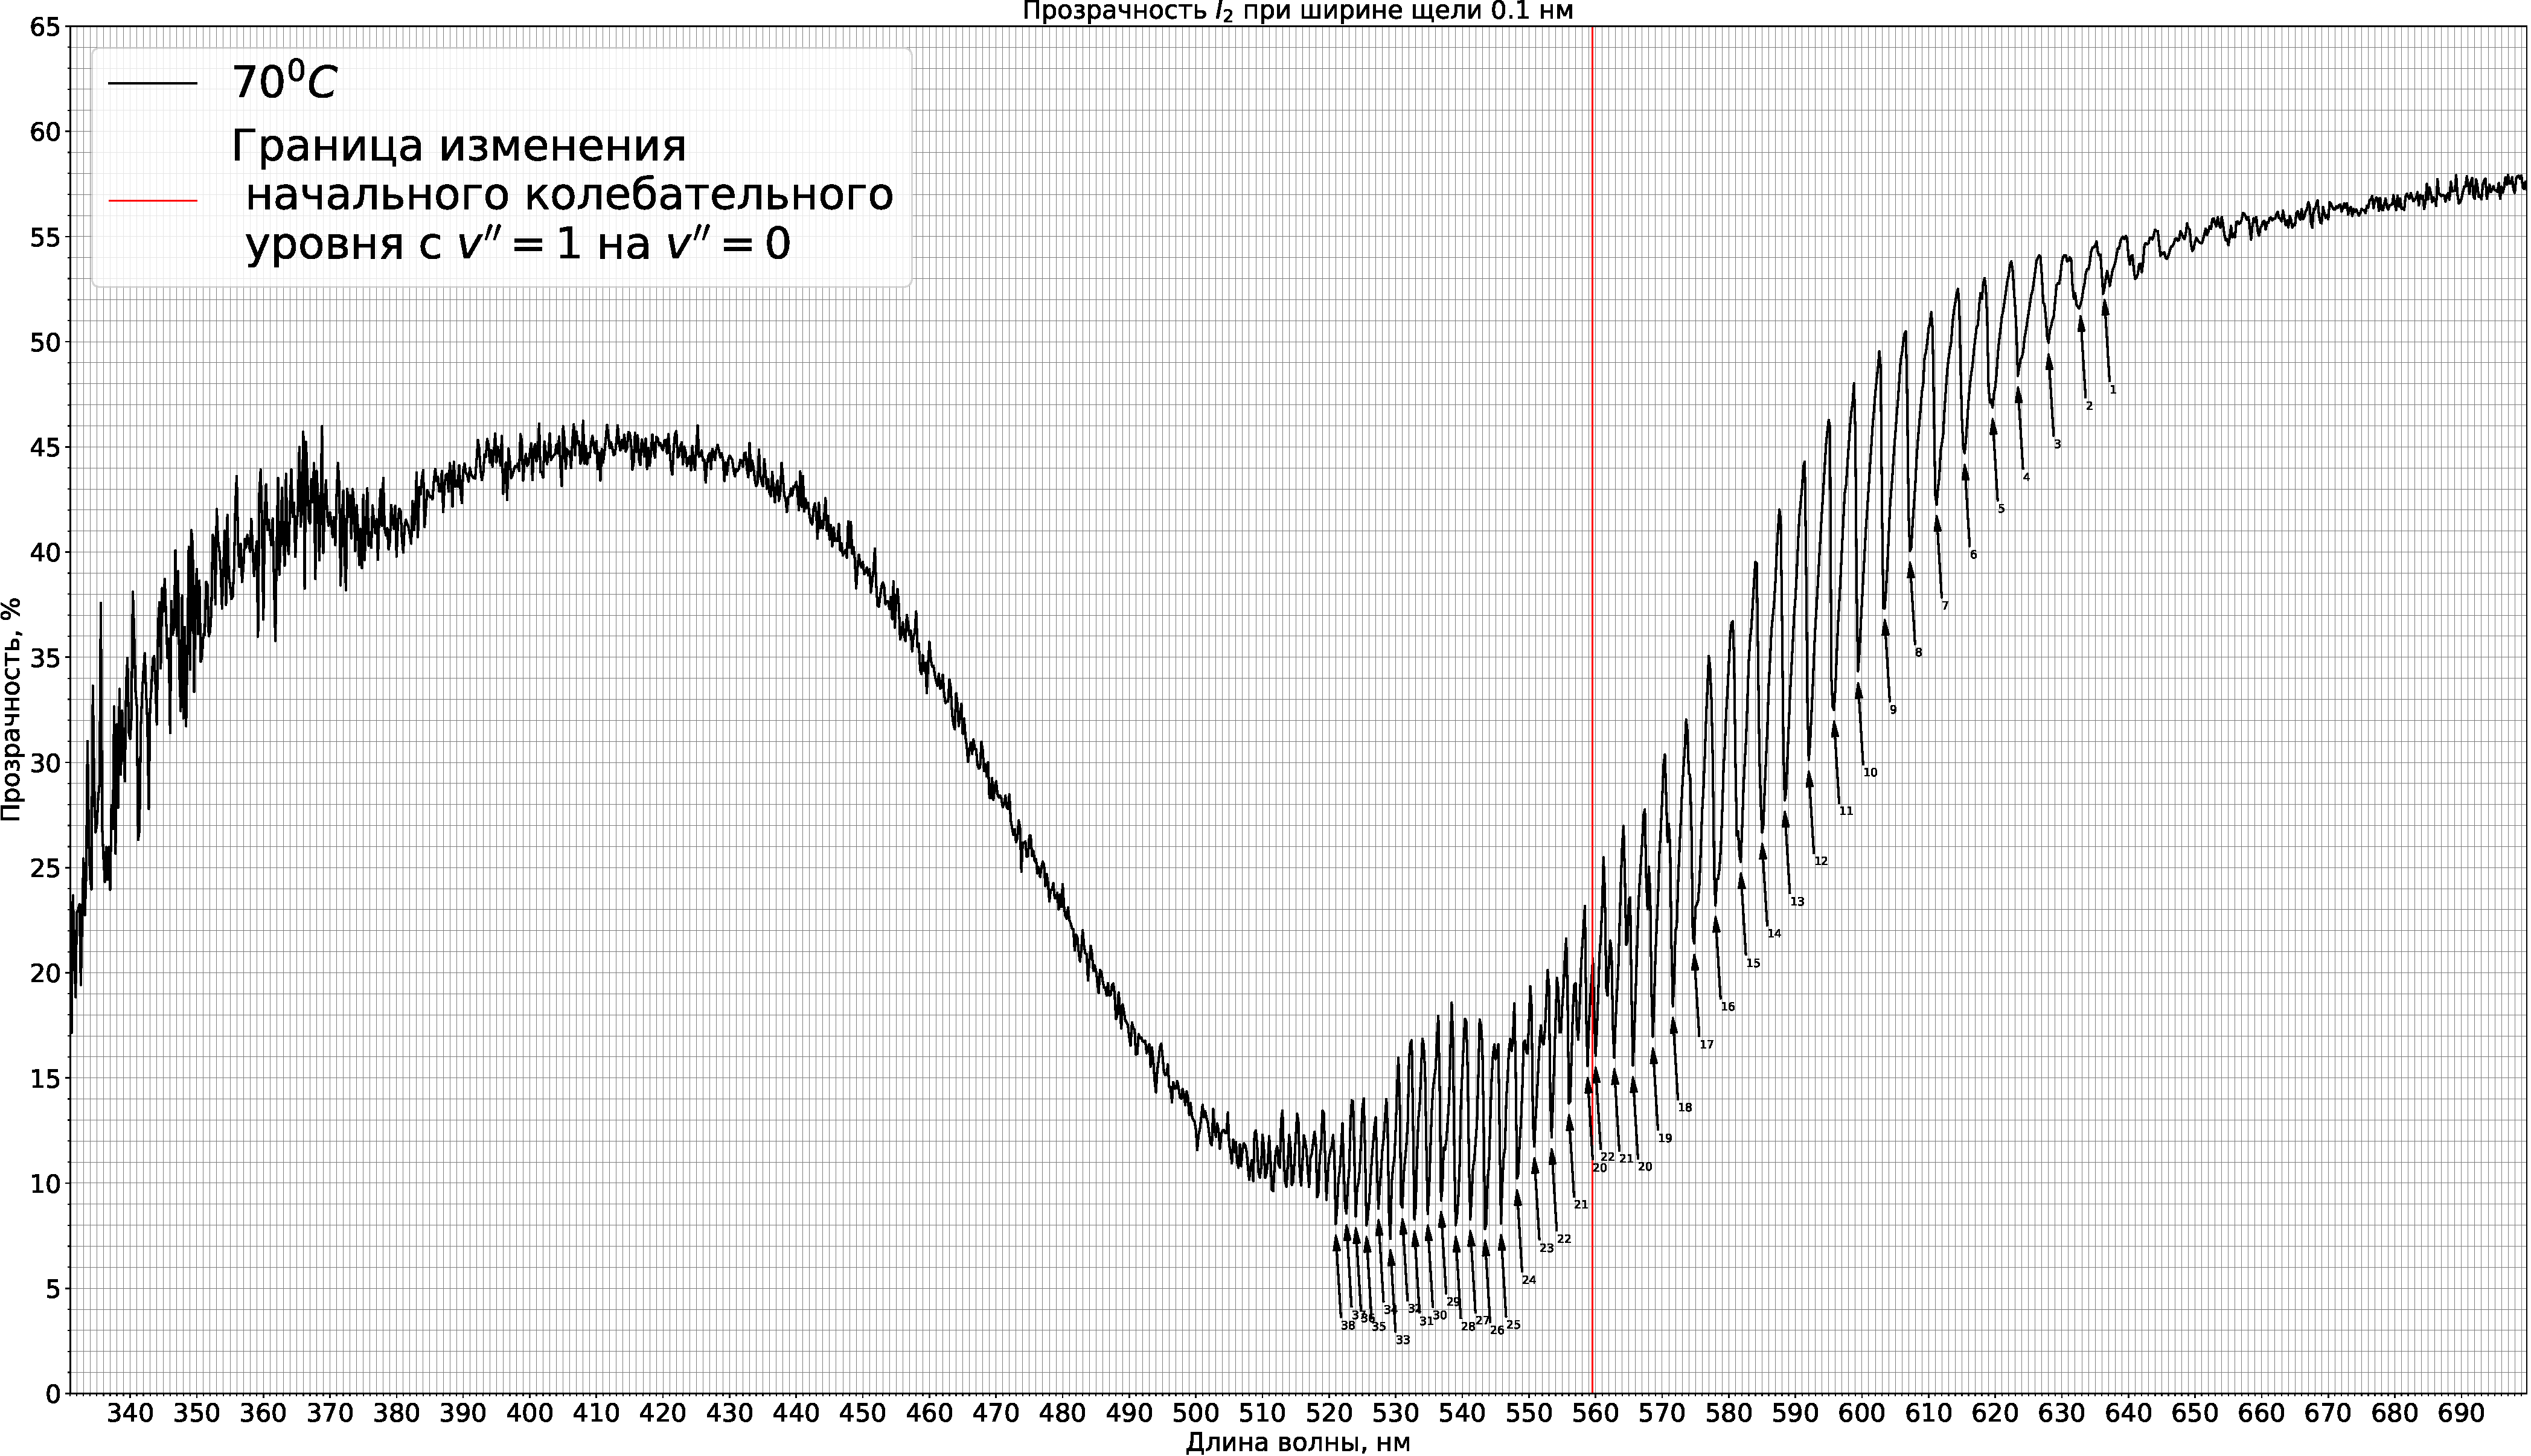
\includegraphics[angle = 90, height=0.87\textheight]{data/long_spectrum}
	\caption{Спектр поглощения молекулы I$_2$}
	\label{long_spectrum}
\end{figure}
На графике видны характерные области для $v'' = 0$ и $v'' = 1$ прогрессий. Заметим, что в области длин волн 380--500 нм поглощение резко падает. Это может быть объяснено тем, что в этой области происходит диссоциация молекул, и дальнейшее поглощение энергии связано с увеличением кинетической энергии атомов.

